% !TEX encoding = UTF-8 Unicode
\pdfoutput=1
%%%%%%%%%%%%%%%%%%%%%%%%%%%%%%%%%%%%%%%%%%%%%%%%%%%%%%%%%%%
%                                                         %
% Title: SISSA Students' Vademecum                        %
%                                                         %
% Authors: SISSA Students' Representatives                %
%          <studentreps@sissa.it>                         %
%                                                         %
% Language: English                                       %
%                                                         %
% Character set encoding: UTF-8                           %
%                                                         %
% *** START OF VADEMECUM.TEX ***                          %
%                                                         %
%%%%%%%%%%%%%%%%%%%%%%%%%%%%%%%%%%%%%%%%%%%%%%%%%%%%%%%%%%%


%%%%%%%%%%%%%%%%%%%%%%%%%%%%%%%%%%%%%%%%%%%%%%%%%%%%%%%%%%%
% Basic class definitions, typesetting, bibliography      %
%%%%%%%%%%%%%%%%%%%%%%%%%%%%%%%%%%%%%%%%%%%%%%%%%%%%%%%%%%%
\documentclass{sissavademecum}


%%%%%%%%%%%%%%%%%%%%%%%%%%%%%%%%%%%%%%%%%%%%%%%%%%%%%%%%%%%
% Actual text                                             %
%%%%%%%%%%%%%%%%%%%%%%%%%%%%%%%%%%%%%%%%%%%%%%%%%%%%%%%%%%%

\begin{document}

\maketitle
\tableofcontents
\newpage

\setlength{\parskip}{1em}


\addcontentsline{toc}{part}{Part 0 - Welcome!}
\chapter{\texorpdfstring{\faGlassCheers\ }{} Welcome to SISSA and Trieste}

Dear first-year PhD students, congratulations on your choice of SISSA for your graduate studies: here in Trieste you will find a welcoming and stimulating environment, for both your academic and your social life. With this document, that is based on the \href{https://wiki.sissa.it/students/index.php/Main_Page}{\textbf{SISSA Students' Wiki}}, we would like to share some tricks with you on how to get the best from your experience here in SISSA and Trieste. \\
From the very beginning, do not hesitate to write to us! Pop over to our \href{http://students.sissa.it/studentscouncil/index.html}{\textbf{website}} in case of need or just for having a look at our activities. Hey, we have a \href{https://www.facebook.com/groups/sissastudents/}{\textbf{Facebook page}} as well! You will find news about official SISSA events, PhD students looking for housemates, stuff on sale, discussions about ongoing issues, polls and much more. Finally, if you wish to keep up with the news and receive important notifications directly on your smartphone or laptop, subscribe to our \href{https://t.me/joinchat/FVSmmUDh3_QyYzU0}{\textbf{Telegram channel}} and to the City of Trieste's \href{https://telegram.me/comunetrieste}{\textbf{Telegram channel}}!

\vspace{-0.4cm}


\section{Some History of SISSA}

As of this moment, you might be wondering: where am I now, exactly? Well, you're at the \textbf{Scuola Internazionale Superiore di Studi Avanzati}, or \textbf{SISSA} (International School of Advanced Studies, ISAS), a PhD School founded in 1978 and now located in the Santorio building on top of the hills of the \textbf{Karst} (this is a Slovenian word, in Italian it is ``\textbf{Carso}'') behind the city of \textbf{Trieste}.\\
SISSA used to be located near Miramare Castle, by the sea, next to the International Centre for Theoretical Physics (\textbf{ICTP}). SISSA moved some years ago to the present building, which used to be a hospital for people suffering from tuberculosis (the ``\textit{Sanatorio Santorio Santorio}'' -- it's no joke: you may find a bust of Santorio Santorio in the hall just outside the Cafeteria). The beautiful \textbf{park }surrounding the Santorio building is also owned by SISSA, although it has been made open and accessible to the public since May 2011 -- during certain times, this is still a workplace after all! You should definitively seize the chance to have a walk around it, when ``\textbf{Bora}'' (the strong, extremely cold wind that sometimes blows in Trieste) is at rest!


\section{Doing Science in Trieste}

Apart from SISSA and ICTP, Trieste and its surroundings host many other scientific institutions, like \textbf{INAF-OATS }(the Astronomic Observatory of Trieste), the \textbf{AREA Science Park} where the biggest Italian collider is settled, \textbf{ICGEB }(International Centre for Genetic Engineering and Biotechnology), \textbf{OGS }(the National Institute for Oceanography and Experimental Geophysics), and the \textbf{University of Trieste}. SISSA collaborates actively with most of these institutes.

ICTP operates a shuttle service to freely transport people from SISSA to ICTP and viceversa. The departure from SISSA is in front of the reception at floor $0$. The schedule can be found \href{https://www.ictp.it/visit-ictp/transportation/campus-shuttle-services.aspx#close}{here}.


\section{Your First Days in SISSA}

Personalise your badge, mailing lists subscriptions, office keys, library account and always check the e-mails!

\noindent For most bureaucratic questions, you can turn to:
\begin{itemize}
	\item the \textbf{Students Secretariat} is concerned with ``general'' problems, like enrollment to the School, housing, tax declaration, etc. (e-mail address: \linkemail{phd@sissa.it});
	\item the \textbf{Secretariat} administrates all issues (missions, booking of lecture rooms, etc.): \href{https://www.sissa.it/scientific-secretariat}{here} is the information relating to the \textbf{Scientific Secretariat} and \href{https://www.sissa.it/articolazione-degli-uffici}{here} you can find the \textbf{general organization} of each office.
\end{itemize}
For more specific issues related to your PhD sector or Area, the people in charge are the following:
\begin{itemize}
	\item the \textbf{PhD Coordinator} (together with the Professors' Council) is in charge of all the administrative issues of your PhD course, for example the coordination of teaching activities, the approval of the plan of studies, the qualifying/progress exams, the approval of missions (when funded by specific PhD course funds), etc.
    \item the \textbf{Area Coordinator} administrates your research Area as a whole.
\end{itemize}


\section{Orientation day}

Each November the students' representatives organise an Orientation Day, an important event where first-year students have the chance to learn about SISSA services and resources, connect with their representatives and gain information about the social activities of the SISSA Club. If you missed this meeting in the current academic year or you just want to have a look at what has been discussed on that occasion, you can find the slides of the last Orientation Days \href{https://www.sissa.it/orientation-day}{at this link} upon logging in with your SISSA credentials.




\chapter{\texorpdfstring{\faHome\ }{} Getting Settled in Trieste (for Foreign Students)}

In the following we will investigate all the mandatory steps needed to settle in Trieste.


\section{How to Get a Tax Code}

The \textit{codice fiscale} or fiscal code is a unique identification number assigned to all Italians at birth by the Ministry of Finance. Any foreigner can request the Ministry to issue a \textit{codice fiscale} without any formality. This code is used to uniquely identify any citizen for tax-related purposes and hence is requested by (almost) any public office as a simple way to uniquely record your data. In order to request the code you must show an identification document (ID card or passport with visa), since the code is generated by combining your birth place, birth date, name and surname.

This code is mandatory for you to open a bank account, rent an apartment etc. If you are a non-EU citizen you should have it in order to get your permit of stay. The easiest way to get this code is to go to the Students Secretariat, where they will help you fill in the forms and make the \textit{codice fiscale} request. Another manner is to go directly to the ``\textit{Agenzia delle Entrate}'' (Income Revenue Authority) Office in Via L. Stock, 4 and ask for a \textit{codice fiscale} there, in this case you should bring your passport and fill in the relevant form.

\vspace{-0.4cm}


\section{How to Get the National Health Insurance}

\href{http://wiki.sissa.it/students/index.php/Health_Insurance}{Here} you can find detailed information. We point out that SISSA can reimburse the cost of the National Health Insurance (Servizio Sanitario Nazionale - SSN for short) subscription via the Students Secretariat (it is handled similarly to the housing contribution).


\section{List of General Practitioners in Trieste}

Upon registration with the National Health insurance, you can choose a General Practitioner from a dedicated list officially provided by the \href{mobility@sissa.it}{SISSA Mobility Office}. Below you can find the most updated version of the General Practitioners who currently speak foreign languages and have been chosen by SISSA's posdocs in the last two years. Feel free to update the list below by expanding it with the names of suitable Practitioners. This may help many of us with our daily life in Trieste!
\begin{itemize}
    \item Dr. Gianna CAPPITELLI (Barcola) - Chosen by most, mothertongue bilingual Italian/French, speaks English fluently (the same holds also for the practice secretary);
    \item Dr. Giuliano ROCCONI (Viale XX Settembre/Via Carducci) - Chosen by many;
    \item Dr. Bruno RUPINI (Via Udine) - Chosen by many;
    \item Dr. Antonio ZAPPI (Viale XX Settembre/Via Carducci) - Chosen by many native English speakers;
    \item Dr. Furio CAVALLIERI (San Giacomo) - Speaks English for sure;
    \item Dr. Enzo PUPPIS (San Giacomo) - Chosen by many Spanish speakers, it is not clear if he speaks Spanish effectively;
    \item Dr. Nives PECAR (San Giacomo + Opicina) - Chosen by Serbian speakers, understands other Balkan/Russian languages;
    \item Dr. Paolo PESCE (Largo Barriera/Ospedale Maggiore) - Chosen by Russian speakers;
    \item Dr. Giancarlo PAOLETTI (Via Udine) - Chosen by Spanish speakers;
    \item Dr. Grazia CEO (Via Mazzini) - Chosen by Spanish speakers;
    \item Dr. Rosanna POGGIOLINI - Chosen by Spanish speakers;
    \item Dr. Piero SIMONITI - Chosen by Spanish speakers; speaks English very fluently;
    \item Dr. Michele SIMONIS - Chosen by French speakers.
\end{itemize}
For those who may be interested, we report here also the name of a pediatrician who speaks fluent English.
\begin{itemize}
    \item Dr. Sonia BERTRAND (Roiano).
\end{itemize}


\section{How to Get (and Renew) the Permit of Stay}

\href{http://wiki.sissa.it/students/index.php/Permit_of_stay}{Here} you can find detailed information.


\section{How to Get a Suitable Bank Account}

In order to receive the deposit of your monthly fellowship from SISSA, you must have a suitable bank account. The suitability of your bank account will depend on where it is located:
\begin{itemize}
    \item In Italy: your account will be suitable;
    \item In a SEPA member state (see \href{https://www.ecb.europa.eu/paym/integration/retail/sepa/html/index.en.html}{here} for an exhaustive list), your account will be suitable, but you may wish to open an account in Italy as well;
    \item In a non-SEPA country (see \href{https://www.ecb.europa.eu/paym/integration/retail/sepa/html/index.en.html}{here} for reference), your account will not be suitable and you will need to open a new account in Italy.
\end{itemize}

SISSA has an agreement with the Opicina branch of UniCredit Banca, located in Piazzale Monte Re, $3/2$, Opicina, which will speed up the process of opening a new account. The documents needed to open a new bank account are as follows:
\begin{itemize}
    \item your Italian tax code (\textit{codice fiscale});
    \item the receipt that the ``\textit{Questura}'' (central police station) gave you when you applied for your permit of stay (\textit{permesso di soggiorno});
    \item certification that you have won a SISSA fellowship;
    \item a SIM card with an Italian telephone number with enough credit to send an SMS.
\end{itemize}

With these documents in hand, you can write to \linkemail{phd@sissa.it} and they will make an appointment at the bank for you.


\section{SISSA's Housing Service}

If you are a foreign student and not sure how to rent an apartment in Trieste, you can ask help to SISSA's housing service (link to its website \href{https://www.sissa.it/housing}{here}), a service managed by \href{http://www.welcomeoffice.fvg.it}{Welcome Office Friuli Venezia Giulia (FVG)}. This is located in the old town centre -- Via dei Capitelli, 960A -- near Piazza Unità d'Italia. It is available for all kinds of support, receives by appointment only and opens on Tuesday and Thursday from $10.0$ AM to $1.00$ PM and from $4.00$ PM to $5.00$ PM (although flexible appointments can be arranged before $10.00$ AM and starting from $2.00$ PM). You can contact it through 
\begin{itemize}
	\item Phone: $+39 040 375 5246$
	\item E-mail: \linkemail{housingsissa@welcomeoffice.fvg.it}
\end{itemize}

At your request, an employee of the housing service will accompany you to visit the rooms or the apartments they propose. Moreover, they will give you advice in order to ensure that you sign a regular rental contract. For more information about rental contracts, please visit this \href{https://wiki.sissa.it/students/index.php/House_rental_contract}{webpage}.

Moreover, the Welcome Office FVG offers free information and personalized support on mobility-related issues to international students and researchers. Students may benefit from a compelling informative \href{link http://www.welcomeoffice.fvg.it/news/}{website} and on-site assistance provided by the local helpdesk in Piazza Unit\`a $4$/b (City Hall - ground floor at Trieste InfoPoint). Furthermore, Welcome Office works together with the \href{https://euraxess.ec.europa.eu/}{EURAXESS centre} in Trieste for the career development of researchers (PhD and Post-Doc) through the organization of training courses, job and recruiting events, workshops on EU funds and opportunities, as well as by offering a whole range of integrated facilities with a view to improving the stay and relocation in Friuli Venezia Giulia and to boost support services already provided by the host institution. 

Once you find a house but realize that you don't have dishes, cutlery, cookware, bed sheets, towels and so on, you can go to AZCASA, a series of shops that can supply all these things to you. If you prefer, on Saturdays and Sundays a bus leaves from Oberdan square towards IKEA in Villesse (a city reasonably far from Trieste): the ticket is about 2 euros and can be bought directly on the bus! For more information, search for ``Shopping bus - Trieste'' on Google.


\section{Asking for residency in Trieste}

If you want to apply for permanent residence in Italy, at \href{https://www.comune.trieste.it/it/servizi-9173/anagrafe-stato-civile-9317/anagrafe-iscrizione-per-residenza-9360}{this} link you find all the instructions needed to ask for the residence registration, the request form to be filled out and additional files listing the documentation needed. In particular:
\begin{itemize}
	\item Attachment A reports the documents requested to non-EU applicants;
	\item Attachment B reports the documentation requested to EU applicants, with a specific section dedicated to students.
\end{itemize}

The residence application should be submitted to \linkemail{variazioneres@comune.trieste.it}. The application receipt is acknowledged by a confirmation of the starting of the necessary administrative procedures. Within 45 days after the submission of the residency application, the Italian traffic wardens are entitled to make an inspective check at your accommodation in Trieste. Therefore, it is highly recommended to specify a preferred time slot for the inspection and an Italian phone number in the application e-mail. If by any chance you are absent on the day of the inspective check, the traffic wardens should leave a notice in your letterbox, through which you can book another check round. After that 45 days have passed since the submission of the application documents, no communications are sent by the Trieste registry office normally, unless your application is rejected.

In case you are in the position of resigning your residency status, you must send an official communication to the very same e-mail address \linkemail{variazioneres@comune.trieste.it}.

More detailed information can be found at \href{http://www.welcomeoffice.fvg.it/practical-info/entry-and-stay/residence-registration-iscrizione-anagrafica/}{this} webpage, as well as by sending an e-mail to \linkemail{mobility@sissa.it}. Beware that this e-mail belongs to the International Relations Office, which in particular is in charge of helping foreign postdocs get their residency (as for them it is mandatory); they are always very willing to help out students who are having problems with their residency request.


\section{Waste sorting in Trieste}

As it is common in the rest of Italy, waste sorting and recycling has become fully operational in Trieste. This means that you can get rid of different types of waste by taking them to specifically coloured dumpsters that you can find on the street. Here is a brief summary of the different dumpster colours and the corresponding purpose:
\begin{itemize}
    \item blue-top dumpster $\to$ plastics;
    \item yellow-top dumpster $\to$ paper and cardboard;
    \item brown-top dumpster $\to$ organic and wet waste;
    \item gray-top dumpster $\to$ undifferentiated waste;
    \item green bell-shaped dumpster $\to$ glass and metals;
    \item yellow containers $\to$ old clothes.
\end{itemize}
Around the city, you can find also small gray bins dedicated to the disposal of batteries: a detailed map of their positions in the city centre can be found at \href{http://wwftrieste.altervista.org/mappapile.shtml}{this link}. \\
SISSA has its own waste sorting policy, too! For instance, green-top bins are destined for paper and cardboard collection, while batteries can be put into easily recognizable column-shaped containers. \\
If you need to dispose of bulky waste, the best practice is to have it picked up directly at home by arranging an appointment with \href{https://www.acegasapsamga.it/clienti/casa/casa_servizio_ambiente/casa_aaa_ambiente_ritiro_ingombranti/32424.html}{AcegasApsAmga}: you will have only to leave the waste next to your building door the day before. \\
In case you need to dispose of other types of hard waste, you should bring it to a waste collection centre. In order to find the one closest to you, you can either visit \href{https://www.acegasapsamga.it/clienti/casa/casa_servizio_ambiente/casa_aaa_ambiente_centri_raccolta/32424.html}{this webpage} or download the app \textit{Il Rifiutologo}, which also provides you with complete information and other details about waste sorting in Trieste. \\
A last piece piece of advice! If not specified directly in your rental contract, beware that there is the possibility that you are required to pay a rubbish collection fee once a year, which usually amounts to order of 100 euros.




\addcontentsline{toc}{part}{Part I - Life at and after SISSA}
\chapter{\texorpdfstring{\faGraduationCap\ }{} Research and Academic Life}

Well, now that you know where you are, you are probably willing to ask: what am I here for? The School's main job is to train you as an independent young scientist. From an academic viewpoint, research in SISSA is divided into three scientific Areas: \textbf{Physics}, \textbf{Mathematics} and \textbf{Neuroscience}. Moreover SISSA has an Interdisciplinary Laboratory which runs the MCS, a master course in science communication, and, jointly with ICTP and the Universities of Trieste and Udine, runs also the MHPC, a master course on high performance computing (see the dedicated \href{https://www.sissa.it/ilas/}{website} for more information).

Being a first year PhD student in SISSA, you are supposed to attend a number of\textbf{ lectures }and take the corresponding \textbf{exams} (except for students in Genomics and Neurobiology), as well as to attend the \textbf{seminars} offered in your PhD course. These will also serve the purpose of letting you know which research topics are active in your Area, and ``who works on what''; as such, participation in your PhD course activities will offer you guidance in your choice of a PhD project.\\
More interdisciplinary seminars, delivered by experts in the fields of research active in the School and open to the whole SISSA community, are organized in the form of the monthly \textbf{SISSA Colloquia}.

Starting from the $2018/19$ academic year, students of SISSA started organizing student-lead seminars called ``\textbf{Interdisciplinary Colloquia}'' (temporary name). The aim of these seminars is to strengthen the bonds of all people working at SISSA (Master and PhD students, administrative and technical staff, professors, etc\dots). In order to do so, scientists and intellectuals with various backgrounds in both science and humanities are invited to SISSA to share their knowledge and expertise. Since these ``seminars'' are organized by students, you all have a very crucial role: you have to suggest speakers and vote on them!

Prepare for the abundant variety of seminars which are given daily here at SISSA, there is something for all tastes! More specific information regarding teaching and seminar activities can be found at the following websites:  \href{https://www.sissa.it/phd-courses}{PhD courses links};   \href{https://www.sissa.it/calendar/event-type/seminar}{Seminars};  \href{https://www.sissa.it/news/colloquia}{General Colloquia};  \href{https://www.sissa.it/news/conferences}{Conferences}; \href{https://www.sissa.it/calendar}{Global Calendar}.


Shortly after your arrival at SISSA, a \textbf{meeting} with the staff and the students representatives of your PhD course will take place, where topics like the above regarding your life as a SISSA student will be discussed.


\section{Your Office, Printing and Binding}

The \textbf{ITCS} (Information Technology and Computing Services) office helps new students get \textbf{SISSA credentials} (username and password). Your account will provide you the possibility to use remote SSH access to SISSA's main cluster servers (example: ssh.sissa.it), an e-mail account and the possibility to register and connect your laptop to the SISSA network in the campus. All the information needed is available on the \href{https://www.itcs.sissa.it}{ITCS webpage}. You can access your account from any computer affiliated with your Area, by logging in with your SISSA credentials.

Moreover, you will soon be assigned your \textbf{office}, in which each of you will have a desk and access to a \textbf{workstation} running a Linux or Windows OS with a lot of software tools already installed, both for scientific (e.g. several LaTeX editors, Mathematica, Matlab, R) and non-scientific (e.g. Skype) purposes. The correct functioning of your machine is a responsibility of the ITCS personnel: contact them if you have any problems or questions. Your computer will obviously be connected to the Internet, but it will be recognized, especially from journal websites, as affiliated to a SISSA account. This will grant you access to many articles (virtually, all the ones you may need), making your bibliographical research much easier. More details on this can be found on the Library website (see page \pageref{sec:Library} for details).

Once you have downloaded your gigabytes of articles, why would you tire your eyes reading them on a screen rather than on paper? You can use SISSA \textbf{printers}, located on every floor. Notice that, as SISSA users, you will have right to unlimited printing, but please do not push it too far! If one of the printers runs out of paper and you are able to replace it by yourself, you can find suitable paper in the \textbf{deposit rooms} which are usually located near the \textbf{toilet} (incidentally, toilet on all floors are marked by yellow walls). \textbf{Photocopiers} are also found near the printers. You can use them to scan your documents and have them sent to you by e-mail in PDF format, following the instructions displayed by the machine. You can also bind the articles that you just printed with binding spirals: you can ask for them at the Store (see page \pageref{sec:Store} for details) and using the binding machine on the 2nd floor, in front of the Students Secretariat. \\
Speaking of printing necessities, you can print the door labels for your office at these links:
\begin{itemize}
	\item \href{https://www.math.sissa.it/content/door-label}{Mathematic Area}
	\item Physics Area
		\begin{itemize}
			\item \href{https://www.sissa.it/sbp/webtools/doorlabel/door.php}{Molecular and Statistical Biophysics  (SBP)}
			\item \href{https://www.statphys.sissa.it/wordpress/?page_id=1684}{Statistical Physics (SP)}, at the bottom webpage
			\item \href{https://drive.google.com/open?id=1cXeavsXzdJGx8aPpN6UYXrCZ6yoPBbuA}{Theory and Numerical Simulation of Condensed Matter (CM)}
			\item \href{https://www.sissa.it/tpp/webtools/doorlabel/door.php}{Theoretical Particle Physics (TPP)}
			\item \href{https://www.sissa.it/ap/webtools/doorlabel/door.php}{Astrophysics and Cosmology (APC)}
			\item \href{https://www.sissa.it/app/webtools/doorlabel/door.php}{Astroarticle Physics (APP)}
		\end{itemize}
	\item Neuroscience Area \textcolor{red}{[Work in progress]}
\end{itemize} 

From the office, you can also make \textbf{free telephone calls to the area of Trieste}, but calls outside the SISSA area have to be authorized by the Coordinator of the PhD course. However, if you have to call someone in the SISSA building, just look up in the \href{http://services.sissa.it/phonebook/index.php?r=site/people}{\textbf{Phonebook}} his/her number and extension. Speaking of telephones, the SISSA building is located very near to the border with Slovenia, so your mobile phone may connect to \textbf{roaming} automatically.


\section{ESSE3 platform and U-GOV service}

In order to ease the administrative business behind your PhD daily grind, SISSA has made the \href{https://sissa.esse3.cineca.it/Home.do}{ESSE3 Portal} available to its students. Accessing your personal area by using the credentials provided upon registration, you can:
\begin{itemize}
    \item take a look at your examination record book (``libretto'' in Italian);
    \item download and print online certificates that you may need e.g. for academic applications;
    \item update your personal data, including those regarding your bank account.
\end{itemize}
If you are wondering about the fiscal side of your administrative experience at SISSA, we have a specific online interface at our disposal. The \href{http://go.sissa.it/cedolini}{U-GOV webpage} allows you to retrieve your monthly pay slips and the annual ``cedolino''. The latter document is also called \textit{Unique Certification}, is released each spring by SISSA's administrative staff and reports your income due to the PhD fellowship with reference to the previous fiscal year. Do not underrate the importance of this document, as it is the main key to obtaining your ISEE certification and possible economic contributions/discounts (jump to Part~\ref{chap:ARDiS} if your interest has been raised).


\section{Missions}

If you plan to attend some interesting schools or workshops outside Trieste, you are entitled to the reimbursement of your expenses by SISSA upon approval. We strongly suggest you read the rules and requirements to be met in order to request a refund: you can find the rules both in \href{https://services.sissa.it/mission/doc/English/ENGLISH_VERSION_REGOLAMENTO_MISSIONI.pdf}{\emph{English}} and in \href{https://services.sissa.it/mission/doc/Italian/2019_REGOLAMENTO_MISSIONI.pdf}{\emph{Italian}}. A manual has been written to answer the most frequently asked questions and to clarify the less clear aspects, and has been edited both in \href{https://services.sissa.it/mission/doc/English/ENGLISH_VERSION_USERS_GUIDE_C_i__PhD.pdf}{\emph{English}} and in \href{https://services.sissa.it/mission/doc/Italian/MANUALE_C_(i)__PHD.pdf}{\emph{Italian}} as well.

The mission forms that you have to fill in can be found on the \href{https://services.sissa.it/online/}{SISSA Web Services page}, into which you can log by your usual SISSA credentials. Before you leave for your mission, fill in the form by \textbf{opening a new mission}. Here you will state which conference you wish to attend and how much money you plan to spend. As a first year student, you may probably want to travel on \textbf{your group's funds}, by selecting the appropriate option, unless you are able to find a different funding source (read below). You will have to fill out this form at least \textbf{one week before} your mission starts, but, as usual, the sooner the better. During your time away, keep all documentation of your expenses (train/plane tickets and boarding passes, receipts, bills and so on); do not forget to also get a certificate of attendance for the event in which you participated. Once you come back, you will have to \textbf{close the mission} through the appropriate online form, with a detailed description of how and how much money you spent, and then hand in the compiled form along with the documentation of all your expenses to the Secretary of your Area (click on \href{http://wiki.sissa.it/students/index.php/SISSA_staff}{this link} for more information).

Starting from 2021, if your mission consists in visiting a faculty abroad or participating in a month-lasting physics school/workshop outside Italy, the minimum number of days for which you can ask an increase of the 50\% of the PhD fellowship is set to 14. Moreover, it is possible to cumulate multiple fundings in order to support missions abroad.

Speaking of funds, you may also be interested in joining one of the national scientific institutes, which can provide a possible alternative source of funding. Some of these different sources include:

\begin{itemize}
    \item \href{http://www.altamatematica.it}{ \textbf{INdAM} (Istituto Nazionale d'Alta Matematica)};
    \item \href{http://home.infn.it/en/}{\textbf{INFN} (Istituto Nazionale di Fisica Nucleare)} and \href{http://www.inaf.it/en?set_language=en}{\textbf{INAF} (Istituto Nazionale di Astrofisica)}.
\end{itemize}

For long visiting periods within the EU (from 3 to 6 months), there is also the opportunity of \textbf{Erasmus Job Placement Fellowships}. The official announcements are forwarded by the Students Secretariat in September-October, with a deadline of about one month. Further information at \href{http://wiki.sissa.it/students/index.php/Erasmus_\%2B_Programme}{this link}.

A contribution towards expenses for training and research activities may be assigned to PhD students enrolled in either their third \textbf{or} fourth year of the course. This contribution is, in particular, aimed to support the self-promotion of students during their search for postdoctoral position. The amount of money given is \EUR{} $1000$ and can be credited \textbf{una tantum} upon \textbf{request} of the student. For more detailed explanation, see the dedicated \href{https://wiki.sissa.it/students/index.php/Training_and_research_contribution}{webpage}.


\section{Teaching at the University of Trieste}

If you want to make some extra money and train your communication skills, a teaching assignment at the University of Trieste is perfect for you. Every year the departments of Trieste's university look for someone willing to tutor their young bachelor students in mathematics and physics. To apply for these positions, you need to speak Italian. In this case, you have to look at the public calls AFC (\emph{bando pubblico Attività Formativa Complementare}) that are uploaded in the \href{https://www.units.it/ateneo/albo}{Albo Ufficiale} of the University of Trieste, usually from 
\begin{itemize}
    \item Dipartimento di Fisica;
    \item Dipartimento di Matematica e Geoscienze;
    \item Dipartimento di Scienze Economiche, Aziendali, Matematiche e Statistiche.
\end{itemize}
These calls usually appear in Autumn (September/October) and in late Winter (February/March), immediately before the beginning of the lectures. Note that usually these departments upload also public calls for teaching activities following D.M. 976/2014; SISSA PhD students \textbf{cannot} apply to these calls. Before applying to these announcements, it is better to inform the Area Council of your reference. Note that:
\begin{enumerate}
    \item first year PhD students cannot participate by national law;
    \item in any case, you can teach for at most 40 hours a year. 
\end{enumerate}




\chapter{\texorpdfstring{\faCogs\ }{} A Look after Your PhD}

What are the opportunities for someone with a PhD degree outside academia? How can SISSA help you look for these opportunities? In order to answer these and other related questions, SISSA has fostered a number of orientation initiatives and personal development opportunities from which its students could benefit in view of their future careers. In the following, you can find a tentatively exhaustive account of all these soft instruments that you should be aware of.


\section{SISSA Alumni Society}

After you get your PhD title, you could want to keep in touch with your PhD travel companions coming from different scientific backgrounds, not only preserving a long-lasting sense of community, but also for being up-to-date with the career paths of your past colleagues. The \href{https://alumni.sissa.it}{SISSA Alumni Society} makes this possible! Each one of the Alumni can inspire the future generations of SISSA graduates by sharing stories of their personal journey, by being a mentor and person of reference for young Alumni continuing their career path in similar areas, as well as by being an ambassador of the School around the world. 
For more information, you can contact them on: \href{https://www.facebook.com/SISSAAlumniSociety/}{Facebook}, \href{https://www.instagram.com/sissaalumni/}{Instagram}, \href{https://twitter.com/AlumniSissa}{Twitter}, \href{https://www.linkedin.com/groups/1761097/}{LinkedIn}.


\section{Valorisation Office and Its Initiatives}

The primary goal of the \href{https://www.valorisation.sissa.it/}{\textbf{SISSA Valorization \& Innovation Office}} is to better motivate SISSA community to invest in the valorisation of its talents and research activities and to try to establish better connections with potential research partners and networks to create a virtuous contamination of ideas in our society. Being at the interface between academia and industry, the V\&I Office job is to inform PhD students and post-docs about placement opportunities, job meetings, self-promotion initiatives, how to protect technologies through intellectual property protections (copyright, patent, etc.) and how to support development and commercialization strategies or create new spin-off and start-up companies, as well as to help students to design their CV and prepare effective job interviews. If all these activities sound interesting to you and you want to know more about them, just jump to their website or send an e-mail to \linkemail{valorisation@sissa.it}.


\section{Coursera}

If you want to start learning programming, improving your hard skills or strengthening your own soft skills and there are no suitable courses at SISSA for your aim, Coursera is what you are looking for. \href{https://www.coursera.org/}{Coursera} in an innovative online learning platform in which people can get access to thousands of lectures on a large amount of topics, especially targeted for those who wants to apply them to new challenges outside academia. Note that some of the courses are for free and some are not. \\
Every year SISSA buys about 200 Campus Plans on Coursera for its students, so that they can attend up to a couple of online courses and earn official certificates upon their completion. If you are interested, wait no more! Send an e-mail to the Students Secretary at \linkemail{phd@sissa.it} asking for this opportunity. \\
Note that third and fourth year PhD students can ask to be reimbursed of the courses using the 1000 euros national budget for self-promotion and self-improvement. For more information, send an e-mail to \linkemail{phd@sissa.it}.


\section{Teaching at the Italian High School}

Outside academia, one of the most attractive careers pursued by students in Italy is high-school teaching. For this reason, Italian universities have made available specific individual, short-term curricula offering aspiring teachers the possibility of gaining the 24 academic credits that are required by the Italian Ministry of Public Education for gaining a permanent teaching role. These courses lie at the crossroads between psychology, pedagogy and anthropology oriented towards educational purposes. As SISSA students, we are given the possibility of attending and giving the exams of such courses (delivered by the University of Trieste) almost for free: only a tax stamp of 16 euros is needed. The subscription period for the 24 Credits Programme ranges approximately from October to December, at the beginning of every academic year. Take a look at \href{https://www.units.it/offerta-formativa/percorso-formativo-24-cfu}{this webpage} if you are interested.


\section{Masters in HPC and SC}

As we all know, science is not only about doing hard-core research, but entails also the development of new, powerful tools serving everyday scientific investigation and, most importantly, public engagement initiatives. \\
SISSA has actualized these two directions by conceiving two professionalizing master courses:
\begin{itemize}
    \item the \textit{Master in High-Performance Computing} (MHPC), an innovative specialization programme that prepares students for exciting careers in the fast-growing field of high-performance computing and its applications (see the dedicated \href{https://www.mhpc.it/}{website});
    \item the \textit{Master in Science Communication} (MSC), the first European master class that train professional figures in the different fields of science divulgation, ranging from journalism and institutional communication to museology, publishing industry and event planning (jump to this \href{https://mcs.sissa.it/}{webpage} for more information).
\end{itemize}
Starting from from the academic year 2020/2021, SISSA has introduced an important novelty regarding the admission to the MHPC: SISSA waves the fee of the Master to its PhD students who are enrolled on one of its PhD courses on the date of the official start of MHPC classes, and to former students who have obtained their doctorate no more than 12 months before the start date of the lessons and that are currently unemployed, for a maximum of \underline{six} exemptions. The exemption is granted to the first three PhD students and to the first three former PhD students that are admitted to the Master, according to the ranking of the admission. Should the number of admitted students or former students be less than three, the exemptions not enjoyed by one of the two categories will be transferred to the other. Beneficiaries of the exemption are required to complete the training course, under penalty of paying € 1.000,00 to SISSA, as a contribution to the training costs. Beware that, if the beneficiary of an exemption is awarded a scholarship that also includes a contribution for the fees (for example, a contribution offered by other research institutions or private companies), the benefit of the exemption is withdrawn and the student is required to pay the balance of the entire fee for participation in MHPC. If this disclaimer has ignited your interest, have a look at how the application process works at \href{https://www.mhpc.it/how-apply}{this link}!


%%% SECTIONS UNDER CONSTRUCTION %%%
%\section{Suggestions to Find a Post-Doc}
%\section{SISSA Contributions to Fund a Start-Up Company}



\chapter{\texorpdfstring{\faUniversity\ }{} SISSA Facilities}

\href{https://www.sissa.it/facilities-and-services}{This} is the page on the SISSA website devoted to facilities and services. In this section, we will give you a brief overview of the basic information.


\section{Library}\label{sec:Library}

Our library is located on the ground floor, ``behind'' the reception. It hosts many physical and electronic books and journal collections on all fields pertaining to the three areas of research led at SISSA: Physics, Mathematics and Neuroscience. Dictionaries, non-scientific books and newspapers can also be found. Using the \textbf{SISSA Catalog} on the  \href{http://library.sissa.it}{\textbf{Library website}} (the central bar ``SISSA Discovery Service'' is a deep research tool that can be ignored at first glance), you can check whether the book you need is currently available: if this is the case, you can either read it in the Library itself, where a number of desks are available and the atmosphere is very quiet, or loan it and take it home with you (you can have up to $5$ simultaneous loans); if the desired book not immediately available because it is loaned by another user, you can still make a reservation; if SISSA's Library does not own what you are searching for, there are several ways to get it:
\begin{itemize}
    \item \textbf{Document Delivery}: filling a specific form, you can request and receive an article or a book chapter (usually scanned) from other libraries and universities.
    \item \textbf{Inter-Library Loan}: you can loan a book from other libraries and universities.
    \item \textbf{Book Acquisition}: you can ask for the acquisition of a new book not present in the SISSA Library. In this case, consider that your request might be rejected if not supported by a professor and that the procedure might take 2-6 months to be processed. 
\end{itemize}

A self-loan service, which can be used also outside working hours, is available upon registration of your badge (see \hyperlink{Badge}{here} for more details). In the FAQ section on the Library website you can find more detailed information about
\begin{itemize}
    \item how to access the loan system (once you arrive in SISSA, you are not automatically authorized to use the library services);
    \item how to manage loans, renew, returns and reservations;
    \item how to find printed books/journals and electronic book/articles;
    \item how to access journal websites with a remote SISSA account from your own PC;
    \item how to access the Document Delivery, Inter-Library Loan and Book Acquisition procedures.
\end{itemize}

In case you cannot find the book that you need at our Library, you can also check the \href{http://library.ictp.it/}{\textbf{ICTP ``Marie Curie'' Library}}. As mentioned above, until a few years ago SISSA and ICTP were very close, so they shared the ``Marie Curie'' Library. Consequently, it hosts a large amount of books not just about Physics, but also in all the research areas of interest in the School. In order to get full access to the ``Marie Curie'' Library services, you need to ask SISSA's Students Secretariat to certify your SISSA affiliation by sending an e-mail to the ``Marie Curie'' Library loandesk.

In the Library, there are two meeting rooms (called Red and Blue Meeting Rooms) that can be booked also by students for collective Skype calls and group meetings: for this service, you have to ask Marina at the loandesk or the Secretariat of your scientific Area (on the first floor).

A bit more advertising! SISSA's library is among those pivotal facilities which allow PhD students to take part in its activities through the 150 Hours programme and, indeed, students' help is most welcome. Give it a thought if you wish to contribute!

Connecting to the web via SISSA VPN's (take a look at the details \href{https://www.itcs.sissa.it/services/network/internal/vpnclient}{here}) allows you not only to download papers published by online journals for free, but also to have privileged access to e-books printed by Cambridge University Press and Springer. Here is a brief summary of how it works.
\begin{itemize}
    \item Until the very end of 2021, SISSA guarantees free access to more and 9900 Cambridge University Press e-books from the Science, Technology and Medicine Collections. You can consult and download the desired chapters of the book you are interested in by surfing on the \href{Cambrige Core home page}{https://www.cambridge.org/core} through a SISSA IP (namely, connecting to the web either from either SISSA itself or through the VPN client).
    \item What Springer has to offer is not free, but looks appetizing anyway. Always through SISSA's VPN, you can connect to the \href{https://link.springer.com/search?facet-content-type="Book"}{SpringerLink platform} and order your own personal printed copy of a Springer Nature e-book for 24.99 euros/dollars, including shipping and handling. This service is called \textit{Springer MyCopy} and is available on thousands of STM (Science, Technology and Medicine) and HSS (Humanities and Social Sciences) e-books. Each MyCopy book comes with a color-printed soft cover and black-and-white printed content, while any included illustrations are monochrome. For more details, jump to \href{https://www.springernature.com/gp/librarians/products/ebooks/my-copy}{this webpage}.
\end{itemize}

SISSA has a special agreement with Springer which allows SISSA's students to buy personal softcover copies of some of the possessed eBooks at a lower and fixed price of 24.99 euros (usually, the most recent published ones). To do this, follow these instructions:
\begin{enumerate}
    \item go to the SISSA Library website and look in the SISSA Catalog for the book in which you are interested.
    \item If the book is an online resource, select \emph{Online resource: Springer} in the right column. Note that you need to be linked in the SISSA network (namely, either a SISSA computer or your laptop connected to the SISSA Internet or your laptop with the SISSA VPN on). 
    \item Select \emph{Buy MyCopy} from the top right of the page. 
\end{enumerate}


\section{Cafeteria}

The Cafeteria is located at the ground floor and offers both \textbf{Bar and Canteen services}. The Bar service is available from Monday to Friday from $8.00$ AM to $7.00$ PM (except during summer). Here you can find a variety of snacks and beverages and, of course, coffee. 

For the residents of Trieste, coffee is not just any beverage! In fact, the residents have such a strong connection with this beverage that they have coined a whole lexicon of terms to indicate several typologies. This short glossary will help you getting the hang of the strange vocabulary used in the typical menu of a caf\`e in Trieste. If you want to make sure you get what you want, you must not take anything for granted! Let's start:

\begin{itemize}
    \item for an espresso, order a \textit{NERO}
    \item for a decaffeinated espresso, order a \textit{DECA}
    \item for an espresso with a splash of frothed milk, order a \textit{CAPO}
    \item for a decaffeinated espresso with a splash of frothed milk, order a \textit{CAPO DECA}
    \item for an espresso with a drop of frothed milk, order a \textit{GOCCIA}
\end{itemize}

All these options may be served in a glass instead of a cup, in which case add ``\textit{in B}{}'' to the end (i.e. for an espresso with a splash of frothed milk in a glass, order a \textit{CAPO IN B}). Note that SISSA bar serves two brands of coffee, \textit{Cibao} and \textit{Illy}: the second one is more expensive. Now you know how to order your coffee in Trieste. 

If you don't know where to drink it, you just have to look around you. The wonderful squares and roads of the town are populated by old literary caf\`es where you can breathe that certain Viennese atmosphere that once inspired writers such as Italo Svevo, Umberto Saba and James Joyce. After enjoying a ``nero'' or a ``capo'', try to answer Mauro Covacich's question: ``Is Trieste a town of writers because it inspires people to play with names - coffee included - or do people play with names here, because it's a town of writers?''. Remember that this is only true for the city and province of Trieste. If you go to Monfalcone and ask for a ``nero'', they will bring you a glass of red wine... So be careful!

The \textbf{Canteen service} is available from Monday to Friday, from $12$ PM to $2.30$ PM They serve a wide variety of meals, including vegetarian options. In principle, you can have whatever you want. There are two types of meals which you can choose from:

\begin{itemize}
    \item ``\textit{Speciale}'' (reduced meal): $\frac{1}{2}$ portion of first course, $\frac{1}{2}$ portion of second course, a side dish, a
    dessert/fruit and a loaf of bread;
    \item ``\textit{Intero}'' (full meal): one full portion of first course, one full portion of second course, a side
    dish, a dessert/fruit and a loaf of bread.
\end{itemize}

\noindent You can have discounts on your lunch! See the \hyperlink{ARDiS}{chapter dedicated to ARDiS} services for more details.


\section{Store}\label{sec:Store}

Remember the days in which you had to buy pens, pencils and notebooks? Well, those days are finally over! On floor $-1$, stairwell C, you will find the \textbf{SISSA Store} (e-mail address: \linkemail{store@sissa.it}), where you can get all your stationery for free. When you need something, just go to the \href{http://services.sissa.it/store/}{Store web page}, choose what you need and send an e-mail specifying the item quantities and codes, your name, your Area and PhD course, and your office number; then go to the store and you will be given what you asked for. Please note that the Store has the following opening hours: Monday to Friday, from $9.00$ AM to $12.00$ PM.


\section{Post Office and Shipping}

Just in front of the Store, you can find the \textbf{Post Office}. You can send all your research-related letters (also registered mail (``lettera raccomandata'' in Italian) just by putting them in the ``Mail Out'' box, without any charge (envelopes can be found at the Store). You can also have mail delivered to you directly at SISSA, and you will find your correspondence in the alphabetized pidgeonholes.

To avoid receiving a huge number of personal packages delivered to the campus, the delivery of packages at SISSA is exclusively authorized for products connected to research and training activities. Small-sized packages not pertinent to SISSA activities will be accepted by the personnel in charge, but no notice will be given to the addressee nor any responsibility will be undertaken for their safe-keeping. If necessary for security reasons (i.e. unknown origin or contents), packages will be opened without requiring recipients' authorization and/or made available to Public Security Authorities.\\
To make the shipping procedure smoother, SISSA has installed an \textbf{Amazon Locker} (called \emph{Edoarda}) at the level $-1$, just in front of the Post Office. If you buy something in Amazon, please send it to the Locker. If not available, wait until it is available again. 


At the Post Office, you can also personalize your \hypertarget{Badge}{}\textbf{badge} with your photo, name, surname and date of birth printed on it. You will receive your badge shortly after your arrival at SISSA, simply ask for it at the Reception. It will grant you access to the external door on the second floor and more generally to the SISSA main building, laboratories and the library outside working hours.


\section{Scala Santa Entry Gate}

Apart from the main entrance in front of the bus 38, it is also possible to reach SISSA Bonomea Campus from the Scala Santa entry gate: whether to enter or to leave, you have to ring the video doorbell and ask the operator to open the gate. To sum up: the Scala Santa gate will always stand closed, except on request from Mondays to Saturdays, from 7.00 am to 8.30 pm.

\section{Prayer room}
There is a room at the 4th floor, in which only one person is allowed to enter at any time, that is possible to use for meditation or praying.

\section{Rules for staying in SISSA after 20}
Due to COVID rules, SISSA is officially closing at 8.00 pm. If you want to stay inside the building longer, you have to write an email to \href{mailto:presidio@sissa.it}{presidio@sissa.it} writing the time that you are expected to leave so that the person in charge knows how many people are in SISSA at any time.

\section{Showers}
It is possible to reach SISSA using human-powered transports in a socially acceptable way. A group of volounteers is allowing to use the showers of the gymnasium building (B5) from 8.15 to 10.15 am. A person must always be present in the gym because of security issues. Users should check before using the showers that a person authorized to open the door is present.


\chapter{\texorpdfstring{\faFutbol\ }{} Extracurricular Activities}

But enough with the boring and serious stuff! SISSA also cares about your leisure activities. Apart from the gym and the music room, these are some other extracurricular activities you can entertain yourself with.


\section{SISSA Club}

The \textbf{SISSA Club} offers you the possibility to attend many different activities which can also be proposed by the students and changed every year. Some examples include \textbf{sports, drawing classes, acting lessons, choir, dancing courses, photography classes, and a weekly cineclub}. 

In the park (more precisely, in the B5 building), you may find the \textbf{Gym}. It is actually managed by the SISSA Club members that organize \textbf{fitness courses}. There you can work out and exercise, following the Latin motto ``\textit{mens sana in corpore sano}{}'' (``a sane mind in a healthy body''). 

\textbf{Language courses}, including Italian for foreigners, are also among the available options in addition to scientific English courses. A subscription fee is required to join the Club: it will also cover your insurance if you participate in the sport activities. The SISSA Club can also admit people that are not in SISSA but want to enjoy time with us. For more information, please visit the \href{http://club.sissa.it/}{SISSA Club website}. 


\section{SISSA for Schools}

SISSA also opens its doors to guided visits to the School and the park for schools (ranging from primary to high school institutions). This project, called ``\textbf{SISSA for Schools}{}'' \ (``SISSA per la Scuola'' in Italian), is organized by \textbf{SISSA Medialab}, a SISSA spin-off company involved in science communication and many different activities. Weekly, seminars and other entertaining activities are offered to children with the aim of popularizing science. With the same aspiration, the ``\textbf{Student day}'' is yearly organized to host about 500 high school students willing to discover SISSA's research topics directly from students and professors. If you are interested in science communication, you are welcome to join the program and become a lecturer or a guide for the tours.  For the volunteers, SISSA Medialab organizes a training course in creative science communication for researchers (usually called ``\textit{Science dialogues}''). You can find additional information \href{http://medialab.sissa.it/sissaperlascuola/en}{here}.


\section{Welcome Day and SISSA Parties}

At the beginning of the academic year, a presentation of SISSA -- probably less interesting than the one you are reading {\dots} -- will take place in the Auditorium (Aula Magna) placed in front of the garden: this is the \textbf{Welcome Day} dedicated to first-year students. This is only one of the many social occasions where you will be able to get to know all your colleagues and new friends from SISSA, like the celebrated \textbf{SISSA Parties}. Remember that, among the secret mottoes of SISSA, there is: \textit{Study hard, party harder!} (The official one is ``ma per seguir virtute et canoscenza'', that is ``to follow virtue and knowledge'', quote from Dante's Inferno.) 


\section{Neuroscience Experiments}

An easy way to get some money and contribute to the advancement of science is to participate in the \textbf{experiments} that your colleagues from the Neuroscience Area conduct every day. These are announced on the Facebook group \href{https://www.facebook.com/groups/144096472323480}{``\textbf{Esperimenti SISSA}''} and also advertised via an e-mail newsletter from time to time; if you choose to help a neuroscientist out, you will be paid for your participation!


\section{SISSA's Music Room}

To look after your ``right side of the brain'', SISSA has also a \textbf{Music Room} located in B5 building (first floor, above the gym) and made available for its students. For the time being, you will find a piano and some equipment you can use with your guitar; it is all free to use and at your disposal. Beware that there could be also a number of personal instruments that other students just leave there, so (as a general rule) instruments already in their case should be intended as personal. In order to access the music room space, you have first to get in contact with \linkemail{davide.venturelli@sissa.it} so as to be subscribed to the Google calendar that will allow you to book the room. Your name will also be communicated to the reception that will give you the keys each time you will have to use the room. Remember to return the keys to the reception after playing or the next in line will not be able to use it.




\chapter{\texorpdfstring{\faFlag\ }{} Student Representatives}

If you are having some issues during your time at SISSA or you are simply curious about how the School works, the \textbf{student representatives} are there to help. Each PhD course has its own representative(s), who sit on the Area Council where all the important matters about your scientific Area are discussed (there are also \textit{supplementary} representatives in order to ensure the quorum is met). You will meet your representative(s) at the \emph{Student Council} presentation at the start of your PhD course. You can find the names and photos of all the representatives on the notice board in the Cafeteria, on the \href{http://students.sissa.it/}{website} and at the end of this section. Do not hesitate to write to them at \linkemail{studentreps@sissa.it} if you have any questions or problems related to your daily life in SISSA.

Collectively, the student representatives constitute the \textbf{Student Council}. The Student Council is an advisory body concerned with decisions related to students' activities in the School, with a particular focus on teaching activities. The Council elects a President and a Vice-President. The President transmits the requests of the Council to the Director and to the Academic Senate, and submits an annual report on teaching activities and students' life in the School during the ordinary meetings of the School Council. The Student Council meets on a monthly basis to discuss all issues which are relevant to the whole student body and to convey those issues to the appropriate committees.

In addition to the student representatives in the Area councils, there are representatives also in the
\begin{itemize}
	\item \textbf{Governing Bodies} of the School, which are the
	\begin{itemize}
		\item \textbf{Academic Senate}, which has the function of proposing general and strategic planning and coordinating the educational and scientific activities of the School;
		\item \textbf{Board of Directors}, which has the power to approve the strategic planning, one-year and three-year financial plans and the personnel planning, as well as to monitor the financial sustainability of School activities;
	\end{itemize}
	\item \textbf{Advisory Bodies} of the School, which are the
	\begin{itemize}
		\item \textbf{School Council}, which is the consultative body that gathers all the School academic personnel (student representatives and research personnel) and technical and administrative personnel;
		\item \textbf{Student-Professor Joint Committee}, which monitors the educational offerings, the quality of teaching and the quality of the services provided to students by the academic personnel;
	\end{itemize}
	\item \textbf{Supervisory Bodies} of the School, which are the
	\begin{itemize}
		\item \textbf{Evaluation Committee}, which is the body in charge of evaluating the quality of the teaching and research activities carried out by the academic personnel;
		\item \textbf{Quality Assurance Unit}, which manages the implementation of the quality assurance procedures according to the guidelines defined by the Governing Bodies.
	\end{itemize}
\end{itemize}

The Student-Professor Joint Committee, the Quality Assurance Unit and the Evaluation Committee work together on the quality assurance system developed by the School. SISSA is indeed dedicated to ensuring the high quality and continuous improvement of its academic standards. The School has developed and maintains periodic internal quality assurance policies and procedures with the involvement of all stakeholders to strengthen the quality culture within the institution. In order to measure the students degree of satisfaction about teaching and research activities, students' services and employability, the School carries out an annual students' survey that is solely for students officially enrolled in PhD courses at SISSA.

For more information about the School quality assurance system visit \href{https://www.sissa.it/qualita}{this website}. You can find more information on the organization of the School's governing bodies on the dedicated \href{https://www.sissa.it/general-organization}{page}.

It is a duty and pleasure for all the student representatives to help you get the best from your experience as a SISSA fellow. Feel free to contact them, either in person or by dropping them a line.

Important updates relevant to students can also be found on a Facebook page managed by the student representatives themselves, click \href{https://www.facebook.com/groups/sissastudents/}{here} for jumping to it.

% --- POSTER OF THE REPRESENTATIVES --- %
\begin{figure}
	\vspace*{-12pt}
	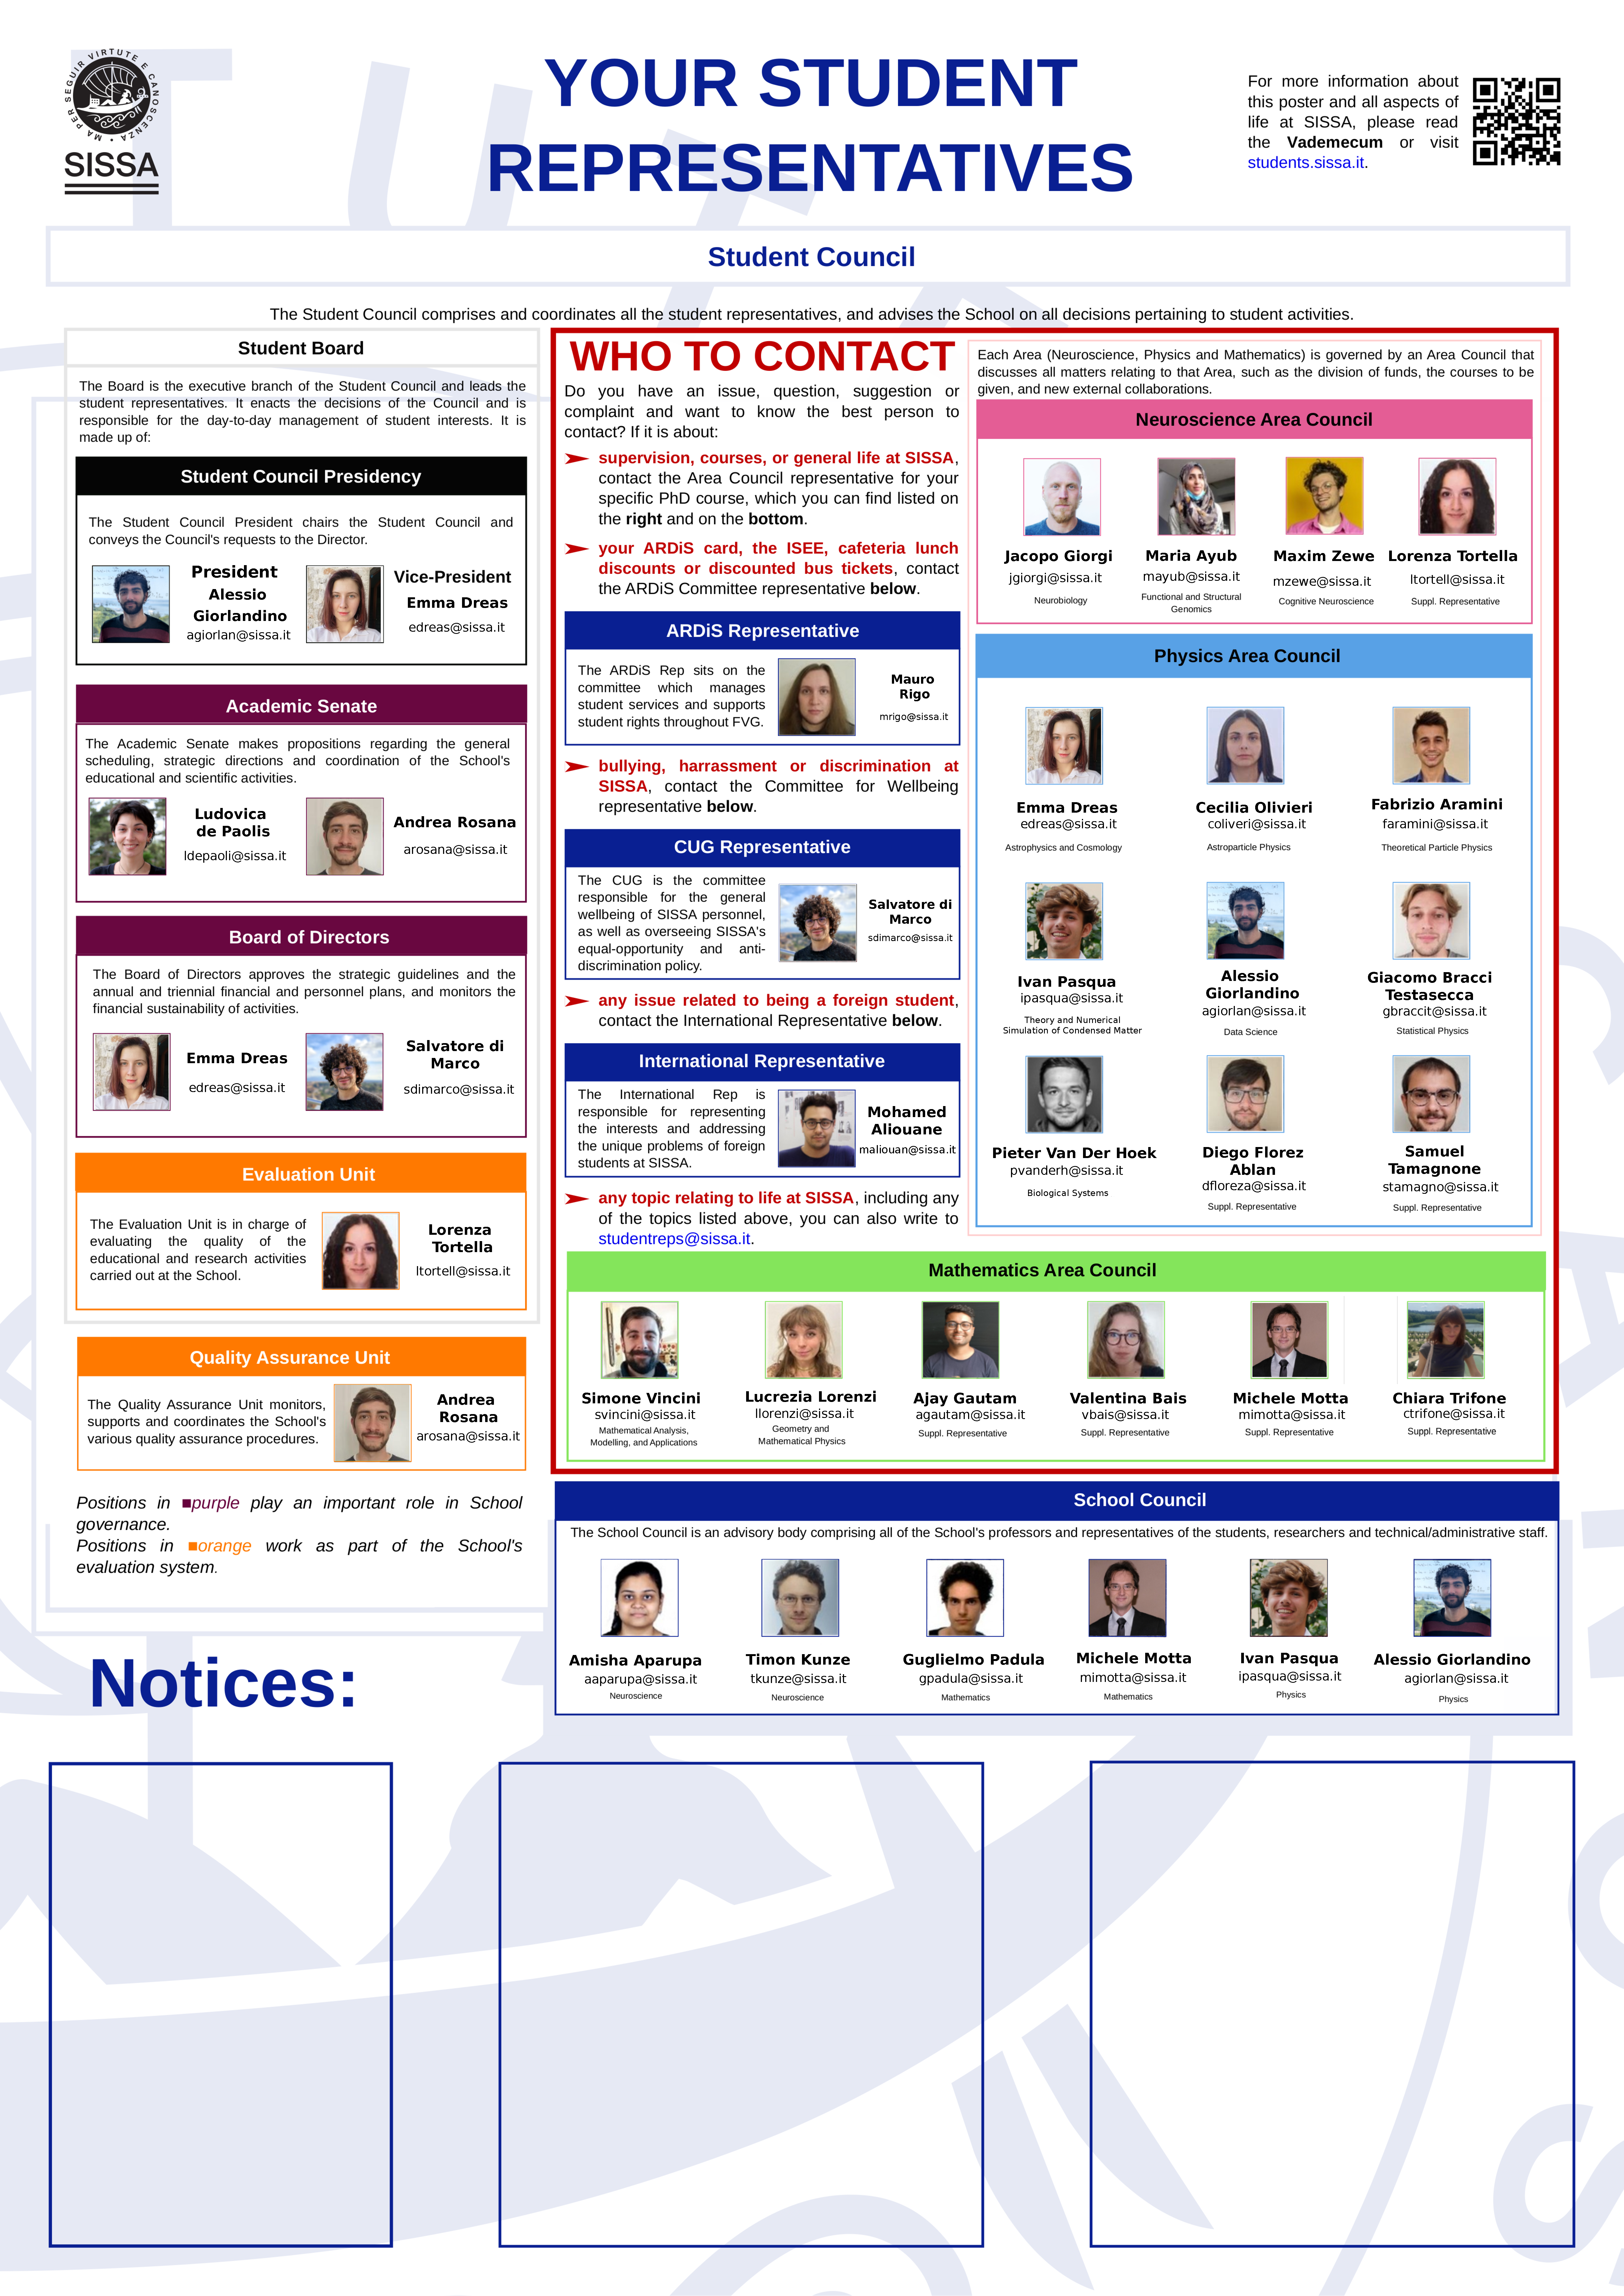
\includegraphics[height=1.05\textheight,center]{StudentPoster}
\end{figure}




\chapter{\texorpdfstring{\faChartBar\ }{}Other Administrative Services}


\section{Media Relations and Communications Unit}

The \textbf{SISSA Media Relations and Communications Unit} (better known as Press Office) is in charge of managing media relations, social media and the SISSA website homepage. It takes care of preparing press releases, press reviews and the development of media products. Moreover, the Unit oversees the School's visual identity and organizes some of the School outreach events. If you are interested in promoting your research in the media, you are willing to take part in outreach initiatives or you have any enquiry concerning communication activities, please write to \linkemail{pressoffice@sissa.it} or contact any member of the \href{https://www.sissa.it/media-and-press}{Media Relations and Communications Unit}. Please also note that the SISSA logo, letterhead and PowerPoint templates are available at \href{https://www.sissa.it/researchers-and-sissa-staff}{this webpage}.


\section{Health and Safety Management}

\textbf{Health and Safety Management} is in charge of evaluating, communicating and preventing workplace hazards. In particular, among all the bureaucratic fulfillments that the School has to implement to guarantee its employers safety, this office is in charge of organizing the mandatory courses for first year student about health security (crucial above all in laboratories) and managing all kind of emergencies (fire, earthquakes, heart attacks, etc.) and possible buildings evacuation. If you need to contact
\begin{itemize}
	\item  a First Aid Operator urgently, you can either call the \textcolor[rgb]{0.06666667,0.33333334,0.8}{911} from any internal SISSA phone or the number 040-3787911 from your personal mobile phone. To report minor accidents and to notify the lack of necessary materials in First Aid Boxes, you can send an e-mail to \linkemail{911@sissa.it}. 
	\item Emergency Evacuation/Fire Protection personnel urgently, you can either call the \textcolor[rgb]{0.06666667,0.33333334,0.8}{555} from any internal SISSA phone or the 040-3787555 by your personal mobile phone. To report issues related to fire starting and situations that you feel abnormal or potentially dangerous (like a fire door that does not close well or by itself) you can send an e-mail to \linkemail{555@sissa.it}. 
\end{itemize}
Remember that in both cases there are about 20 suitably trained people ready to help you. If there is any emergency, please do not call by your self the Italian Number for Emergencies (112), because if an ambulance comes here in SISSA and does not know where to go (there are several buildings and one of them is much bigger than the others) it will not be very useful. The right procedure consists instead in firstly contacting the internal number 911: a trained operator will come to give you support, while the other operators will call and welcome an ambulance at the entrance of SISSA (to bring First Aid Operators straightly where needed). Remember further that throughout the European Union the abuse or simply the joking call of these numbers is considered illegal by law. 
In SISSA there is a portable defibrillator that can be used only by authorized personnel. However, since people can enter the building also during the weekends when the First Aid surveillance is not present, it is good to know that it is installed at floor $0$ diametrically opposite with respect to the reception. NEVER TOUCH THE DEFIBRILLATOR IN ABSENCE OF AN EMERGENCY because it is alarmed and linked with the ambulance station. Any abuse will be pursued (there are cameras!). 

Remember also that if you want to bring from home some additional chairs, tables, electric boilers and so on, they have first to be approved by this office. For any other issue you can contact the Health and Safety Management at \linkemail{safety@sissa.it}. More info can be found on this \href{http://www.sissa.it/safety}{website}.




\chapter{\texorpdfstring{\faShieldVirus\ }{} SISSA During the COVID-19 Saga}

In this chapter, you can find essential information on the procedures that SISSA has employed in order to safeguard everybody's health in these tough times. Moreover, we also provide some useful tips with the hope of making your work at SISSA's facilities as comfortable as possible! \\
This information is summarised below in the form of an FAQ. Visit SISSA's \href{https://www.sissa.it/news/covid-19-access-sissa-and-schools-activities}{webpage} for more details.


\section{Can I Access SISSA?}

According to the actual Italian regulations, the Green Pass will be compulsory for all the academic personnel, including professors, administrative technicians, PhD students and research fellows, in order to gain access to SISSA and all its facilities, starting from September 1 until December 31 (2021). More precisely:
\begin{itemize}
    \item from 23/08/2021 to 31/08/2021, the Green Pass will have to be shown to the canteen personnel if you want to have lunch by sitting at the tables inside;
    \item from 01/09/2021 on, you will have to show your Green Pass to the receptionist as a mandatory requirement.
\end{itemize}

{\small
\begin{tcolorbox}[breakable, enhanced, sharp corners, colback=green!30, colframe=green!80!blue, title=Obtaining the Green Pass]
\paragraph{\small For those who got the COVID vaccine in Italy}
\begin{itemize}
    \item If you have received the AUTHCODE from the Italian Ministry of Health via SMS or e-mail, you can use it to recover the Green Pass by filling in the online form that you can find at \href{https://www.dgc.gov.it/spa/public/home}{this link}, keeping your ``Tessera Sanitaria'' (the plastic TEAM-EHIC card) at hand.
    \item In case you did not receive the AUTHCODE but you hold the Tessera Sanitaria, you can obtain the former \href{https://www.dgc.gov.it/spa/public/reqauth}{here} by inserting:
    \begin{enumerate}
        \item your Italian fiscal code;
        \item the last 8 digits of your Tessera Sanitaria (rear side of your TEAM-EHIC card, field 8 – ``Numero di Identificazione della Tessera'');
        \item the reason for request: ``Vaccinazione'' (Vaccination) or ``Certificato di guarigione'' (Recovery Certificate) or ``Tampone'' (Swab);
        \item the date of the event (the time of the last vaccination/swab shot or the date of the end of isolation following a COVID infection communicated by your General Practitioner or SISSA's Prevention Department).
    \end{enumerate}
    Alternatively, you should be able to retrieve a copy of your Green Pass from either pharmacies or your General Practitioner. In particular, we recommend to address ``Farmacia Al Cammello'' (Viale XX Settembre 4) as a convenient place that provides this service.
    \item If you are enrolled in the Italian Healthcare System, but you never received the TEAM-EHIC health card, it is possible to ask the health district to which you belong to send you a preprint of your Tessera Sanitaria displaying the number of the card and its expiry. You can contact either \linkemail{mobility@sissa.it} or \linkemail{phd@sissa.it} for assistance.
    \item Regarding those who do not hold the Tessera Sanitaria because they are not enrolled in the Italian Healthcare System, they can go to \href{https://www.dgc.gov.it/spa/public/home}{this link} and:
    \begin{enumerate}
        \item select ``Utente non iscritto al SSN vaccinato in Italia'';
        \item insert their Italian fiscal code;
        \item specify the date of the last vaccination shot;
        \item select the desired language for the certificate.
    \end{enumerate}
    Finally, you should be able to obtain the certificate by clicking on  ``Recupera Certificazione''.
\end{itemize}
\paragraph{\small For those who got the COVID vaccine abroad}
\begin{itemize}
    \item If you are an EU citizen, remember that the Green Pass (EU digital COVID Certificate) issued by individual states is also valid in Italy.
    \item We recommend to non-EU students to bring with them to Italy the documentation available to them and to arrange for the swab examinations and quarantine measures required by international and Italian standards, see \href{https://www.salute.gov.it/portale/nuovocoronavirus/dettaglioContenutiNuovoCoronavirus.jsp?lingua=english&id=5412&area=nuovoCoronavirus&menu=vuoto}{here} for more details.
\end{itemize}
\end{tcolorbox}
}

Aside from the constraint of possessing the Green Pass, all SISSA students are allowed to access the campus without specific authorisation. Within the School's opening hours, you can carry out both individual and lab-based research activities. Of course, common sense has to be applied! As always, we must keep a safe distance between each other and avoid grouping up. For this reason, you are strongly encouraged to work from home, unless coming to SISSA turns out to be strictly necessary or essential for your working well-being. Keep in mind that, as soon as you access SISSA, you MUST register both your entrance and leave online at \href{https://services.sissa.it/PresenzeWeb/}{this link} by inserting your SISSA credentials. \\
Note that the use of spaces for research activities must comply with safety standards (e.g., distancing, use of PPE, etc.). So check for the presence of other people in shared offices and laboratories ahead of time, and book the facilities and common areas: in this way you will be able to work in peace and safety. \\
If you have medical conditions which put you at a higher risk for COVID-19, please follow the directions provided by the Human Resources Office (e-mail: \linkemail{risorseumane@sissa.it}) and consult your healthcare provider (general practitioner or specialist) or SISSA's company doctor.


\section{How Can I Get to SISSA?}

\begin{itemize}
	\item \textbf{By private vehicle or on foot} - The use of private vehicles must include only the presence of the driver if possible; if you want to bring someone with you, both of you must wear a facial mask or other protective equipment for covering your nose and mouth. During the trip, avoid the use of air conditioning and especially the recirculation function. These limits do not apply if vehicle occupants are cohabitants. It is recommended to arrive at SISSA between 8 AM and 8.30 AM to avoid creating long queues to enter with those using the private shuttle (see below).
	
	\item \textbf{By the SISSA shuttle} - If you do not have your own means of transport, or you prefer not to use it, you can use the shuttle service that SISSA has set up due to the COVID-19 emergency. The shuttle departs from the city centre and operates from Monday to Friday, excluding public holidays, with the following times and stops:
	\begin{itemize}
		\item Inbound: 8:00 AM (Largo Barriera) - 8:05 AM (Piazza Oberdan) - 8:30 AM (SISSA)
		\item Inbound: 8:45 AM (Largo Barriera) - 8:50 AM (Piazza Oberdan) - 9:15 AM (SISSA)
		\item Outbound: 7:00 PM (SISSA) - 7:25 PM (Piazza Oberdan) - 7:30 PM (Largo Barriera)
	\end{itemize}
	Remember that bookings are compulsory and must be made before Thursday 8 AM the week in advance. On the shuttle, you must wear suitable protective equipment for covering the nose and mouth and respect a one-meter safety distance at least. In order to allow for social distancing, the shuttle will have limited capacity: only one person can use a seat row, with the exception of spouses or cohabiting family members. In the latter case it is sufficient to book 1 seat. \\
	You can reserve your place on the shuttle \href{https://sissa-my.sharepoint.com/:x:/g/personal/tomicich_sissa_it/EQLzW_4F4-lGtuPXJdC9qYgBIXrrV-smwd4T0KILQIp_nw?rtime=GPG4zOFM2Ug}{here}. \\
	In case of emergency, you can get in touch with the transport service at 040 7795959 (until 2 November). From 4 November on, please call the number 335 6908396.
	
	\item \textbf{By public transport services} - As a (riskier) alternative, the bus line 38 is still active, while the bus number 64 will reach SISSA as soon as the extension of the square in front of the SISSA entrance has been completed.
\end{itemize}


\section{How Should I Behave Inside SISSA?}

The maximum number of people who may be present at the same time in each shared room has been fixed for all areas in the main building, based on the overall amount of protection devices offered by SISSA to prevent the contagion, the available space, the time of stay and the activity carried out in a specific workplace. \\
To avoid the so-called ``close contact'', it is necessary to ensure a low density of people and the respect of a minimum interpersonal distance of: 1 metre in transit areas (corridors); 2 metres in ``critical'' rest areas (coffee-break areas, smoking areas, etc.) and, unless otherwise specified, in common areas (including offices with more than one person). Note that a ``close contact'' is defined as a contact that occurs in a restricted environment (e.g. office) continuously for 15 minutes or more with an interpersonal distance of less than 2 metres.


\subsection{Masks, Distances and Hygiene Measures}

Keep a safe distance of at least 1 metre. In the corridors, on the stairs, in the bathrooms and in all common areas it is always recommended to wear the surgical mask provided at the entrance or the one in your possession, if considered suitable by the reception staff. Reduce your movements inside the SISSA building to those that are really necessary for your activity. Wash your hands frequently with soap and water, or alternatively with the dedicated cleansers placed on each floor of the School.


\subsection{Cleaning the Workstation}

Do not forget to clean frequently your desk and your workstation by means of the appropriate detergents. Be especially careful to clean well the infamous mouse-keyboard couple.


\subsection{Ventilation of the Premises}

Finally, it is a good idea to aerate your office as often as possible, so as to reduce further the probability of infection transmission.


\section{What About the Bar and Canteen Services?}

\begin{comment}
As of \today\ the take-away service offered by the canteen is operative in a limited fashion, offering sandwiches, piadinas, pizza slices, salads and hot meals as well.

Meals must be booked before 11 AM and collected between 12 PM and 1:30 PM. Bookings can be made:
\begin{itemize}
	\item through \href{https://www.sissa.it/cafeteria}{this link};
	\item by e-mailing \linkemail{ristobar@sissa.it};
	\item by using the paper register at the Reception.
\end{itemize}

If you are interested in receiving updates and communications from the canteen service via e-mail, you can subscribe to the cafeteria mailing list. This can be done by filling out the form that you find at \href{https://go.sissa.it/cafeteria}{this webpage} or by sending an e-mail from the address you want to subscribe to.
\end{comment}

As of \today\ the bar is fully operational and open from 8:00 to 15:00, while the canteen is open from 12:00 to 14:00.

You can eat plated canteen food in the canteen by booking a specific time and place beforehand at \url{https://services.sissa.it/mensa/}. You can also get take-away meals (but \textbf{not} eat them in the canteen, even if you have booked a table) even without booking them in advance.

If instead you prefer to get takeaway sandwiches/piadinas/salads, you have to book them in advance (by 11:00) in one of the following ways:
\begin{itemize}
\item on \url{https://www.sissa.it/cafeteria}
\item by sending an e-mail to \linkemail{ristobar@sissa.it}
\item via the paper register at the reception
\end{itemize}
Sandwiches/piadinas/salads can then be collected at the canteen from 12:00 to 14:00.


\section{Where Can I Retrieve Information on the Current Library Rules?}

Luckily, everything has a place in this world. \href{https://library.sissa.it/new-library-timetable-rules}{Here} you will find all the latest news on the status of the Library services.


\section{Smart Working Toolbox}

We list below some useful tips and reminders that hopefully could make your research activity at home more comfortable and less tiresome.
\begin{itemize}
	\item Did you know that SISSA provides each member of its academic staff with a Basic Zoom account for free? This allows you to organize virtual meetings with no time restrictions due to the number of people participating (as it occurs for the free subscription). Visit \url{https://www.itcs.sissa.it/lecturesonline} for more details!
	
	\item Not only Zoom, but also Overleaf has a special agreement with SISSA. You can claim your free Overleaf Professional account by signing up with a SISSA e-mail (or by adding it to an existing Overleaf account). Notice that a Professional subscription poses no limits on the number of collaborators which you can share your projects with! More info: \url{https://www.overleaf.com/edu/sissa}.
	
	\item During your everyday research activity, you may want to access the SISSA network remotely. Possible reasons: necessity of connecting to your workstation, extreme need of computational resources on the Ulysses cluster, exploiting the opportunity of having direct access to scientific papers (otherwise protected by paywalls) through the holy SISSA identity key. What you need is to establish a VPN remote connection with the SISSA internal network: follow the instructions at \url{https://www.itcs.sissa.it/services/computing/networkaccess}.
	
	\item Other tools that can help you get access to scientific papers while you are off-campus are also \href{https://scholar.google.com/intl/en/scholar/help.html\#access}{Google Scholar's Off-Campus Access}, that works by storing your library subscriptions for 30 days when you visit Google Scholar while on campus, \href{https://scholar.google.com/scholar_settings?sciifh=1\&as_sdt=0,5\#2}{Google Scholar's Library Links}, that lets you add a SISSA Library link next to every search result, and awesome free and open-source (fully legal) browser extensions like \href{https://unpaywall.org}{Unpaywall} (Chrome, Firefox), \href{https://www.oahelper.org}{Open Access Helper} (iOS, Safari on MacOS, Chrome, Firefox) and \href{https://openaccessbutton.org}{Open Access Button} (Chrome, Firefox, or by manually entering the DOI). If you also have a UniTS account, Open Access Helper lets you automatically use its EZProxy (more details \href{https://www.oahelper.org/ezproxy/}{here}) by just looking for ``units'' during the initial configuration.
	
	\item In these challenging times for our daily as well as academic life, SISSA has taken advantage of the Campus Initiative of Coursera, the leading platform for online learning. We encourage you to take a look at the courses available within the SISSA-Coursera agreement by registering at \href{https://www.coursera.org/programs/sissa-on-coursera-dkw8c}{this link} by using your SISSA e-mail. Should you find one or more courses that you wish to follow, please send an e-mail to the Students Secretariat (e-mail: \linkemail{phd@sissa.it}) in order to have your account activated. Just a notice: some students reported that one needs to complete a course to have the possibility to subscribe to another one. You will not able to follow two different courses at the same time under the actual license rights.
	
	\item What would you say if we told that you are allowed to borrow the monitor of your workstation for the benefit of your home-made research? To do so, you have to write to prof. Antonio Lanza (e-mail: \linkemail{lanza@sissa.it}) with the inventory number of the monitor that you wish to get on loan. Make sure that the coordinator of your PhD sector is CC'd in your e-mail!
\end{itemize}


\section{The Final Piece of the Puzzle: Your Feedback!}

We representatives are deeply aware of the continuing difficulties regarding your daily relationship with PhD-related activities, ranging from keeping in contact with your supervisor (a tough challenge in itself, sometimes) to even just managing to do some clean research without thinking excessively about the current situation. \\
Do not hesitate to contact us should you have any problem regarding your PhD life, even if you do not understand some boring, bureaucratic stuff and you feel the need for some advice. We are still here for bridging the gap between your needs and the current workflow of SISSA.




\addcontentsline{toc}{part}{Part II - Discounts, Support and Contributions}
\chapter{\texorpdfstring{\faFileInvoiceDollar\ }{} INPS - Welfare Benefits}
\label{sec:gestione_separata_inps}

Even though for the Italian law you are regarded as a student and not as a worker (the money you receive are technically speaking a fellowship and not a salary!), part of your fellowship is automatically monthly given to INPS, the \emph{National Institution for Welfare Benefits}, where they accumulate it for your future pension. In order to \textquotedblleft get access to this money \textquotedblright\, (and actually many other benefits linked to possible serious illnesses or pregnancies), you must be registered to ``\textbf{Gestione Separata}'', a specific pension fund administered by INPS. The deadline to subscribe to ``Gestione Separata'' is $30$ days starting from the day on which SISSA notifies you of your admission to the PhD program. \\
\indent To subscribe to ``Gestione Separata'' you have to follow \href{https://www.inps.it/myinps/default.aspx?accessoinps=1}{this link} and log into your INPS personal webpage (using your INPS PIN number or SPID), then subscribe to ``Gestione Separata'' under the contributor category named ``Parasubordinato''. If you have already been registered to ``Gestione Separata'' (for example if you had a $150$-hours contract with an Italian university during your bachelor's or master's studies), you don't need to subscribe again and in that page you will just find the past contributions. \\
\indent To get your SPID code, follow the information that you find at \href{https://www.spid.gov.it/en/}{this link}. Note that it can take up to a few weeks to get your SPID number; therefore, the sooner you do it, the better it is. If you already have an INPS PIN, you do not need to get a SPID number but it is recommended. \\
\indent Students who are forced to interrupt their activity due to \textbf{illness}, \textbf{severe personal problems} or \textbf{pregnancy} may be granted a contribution equal to $70\%$ of the fellowship for a maximum period of $5$ months. However, if you are working in a SISSA lab, in case of pregnancy your fellowship freezes starting from the day you notify the Students Secretariat and the Director by sending them a certificate vouching for your pregnancy. You will get a contribution equivalent to the $70\%$ of the scholarship starting from the day of the notification of your pregnancy and ending seven months after the birth of your child. In addition, the date of your PhD defense is postponed by the appropriate length of time. \\
\indent Eventually, if after your PhD discussion you do not have a job, INPS will pay you a little amount of money (about 900 euros monthly) for at most six months or until you find a job. For more information, \href{https://www.inps.it/prestazioni-servizi/dis-coll-indennita-mensile-di-disoccupazione/}{look here}. 




\chapter{\texorpdfstring{\faHandHoldingUsd\ }{} SISSA Support and Contributions}

\vspace{-0.4cm}


\section{Rent Expenses}

A contribution towards \textbf{rent expanses} for students with a regular (registered) contract living in the province of Trieste (with a different domicile with respect to their family of origin). Every year the requests for the annual contributions towards living expenses must be submitted to the Students Secretariat no later than July $31$st through an ad-hoc form provided by the Secretariat itself; those who submit the request by July $31$st and have a rental contract that does not cover the entire period of the current year may subsequently (but not later than December $31$st) submit a second request to integrate it with details on the new rental contract or its renewal in order to cover the remaining period. The entire contribution will be paid in September. For those who submit an integration request, a second payment will be made by January/February in the following year. Students who are starting their first academic year will have to submit the application for the living expenses contribution no later than December $31$st in relation to the first year of the PhD. The contribution for the period from the beginning of the academic year to December will be paid by the end of February in the following year. All the details will be given to you by periodic reminders sent by the Secretariat and you can already find the dedicated form \href{http://wiki.sissa.it/students/index.php/Contribution_towards_living_expenses}{here};
 

\section{Health Care Expenses}

A contribution towards \textbf{health care} expenses (especially dental care); further information is available in \href{https://www.sissa.it/_media/documenti/english_regolamento_interventi.pdf}{English} and in \href{https://www.sissa.it/_media/documenti/regolamento-assistenziale.pdf}{Italian};


\section{Laptop Contribution}

A \textbf{laptop} contribution, consisting in \EUR{} $400.00$ maximum for PhD students enrolled in the first and second years and \EUR{} $300.00$ maximum for PhD students enrolled in the third year. The deadline for the laptop purchase and for submitting the request is October $31$st every year. The bonus will be awarded only once and shall not exceed the price of the laptop. For further information, please visit the dedicated \href{http://wiki.sissa.it/students/index.php/Laptop_contribution}{webpage} on the SISSA Wiki (note that contrary to what the Wiki says, it \emph{is} possible use the laptop contribution to purchase a tablet);
    

\section{Part-time positions for students}

\textbf{Part-time positions for students}($150$ Hours). Students are paid \EUR{} $10.30$ per hour working actively in various tasks at the base of life in SISSA, lasting from $50$ to $150$ hours depending on your availability, such as taking part in the Library administration, keeping the SISSA webpages updated, and so on. This income is tax-free. \textit{First year students cannot apply}, but keep this in mind in view of the following years. You can find more information \href{http://wiki.sissa.it/students/index.php/150_hours}{here};


\section{Contribution for flying back home}

A \textbf{contribution for non-EU students to travel back home}. The maximum amount of the contribution is \EUR{} $500.00$. This can be used only once during the PhD and after two years of work at SISSA (i.e. third or forth years students only). The capital city of the homeland must be more than 1000 km far from Trieste. In order to get the contribution, you should fill in the relevant form, enclose a copy of the travel receipt and your boarding pass and bring them all to the Students Secretariat. For more information visit this \href{http://wiki.sissa.it/students/index.php/Travel_grant_contribution}{webpage};
    
   
\section{Kindergarten}

The ``\textbf{SISSA per i piccoli}{}'' Kindergarten is open to all SISSA staff, including students, to take care of your children during working hours. For further information, see the dedicated \href{https://www.sissa.it/kindergarten}{webpage}.
   
    
\section{Registration to SSN}

Non-EU students are entitled to a reimbursement of the amount of money paid to register with the \textbf{Italian national health system}, up to a maximum of \EUR{} $198$ per year;
    



\chapter{\texorpdfstring{\faTags\ }{} ARDiS Support and Contributions}
\hypertarget{ARDiS}{}
\label{chap:ARDiS}

\href{http://www.ardiss.fvg.it}{ARDiS} is the agency run by the Regione Friuli Venezia Giulia which provides students with services like cafeteria and public transport discounts or psychological support. As you are regarded as a student by the Italian law, you have to pay every year the annual Regional Tax on Higher Studies (ARDiS tax for short); more information will arrive by e-mail from the secretaries at the beginning of every academic year. Note further that to enjoy some of the ARDiS discounts you have to get your ISEE (``\emph{Indicator of the Equivalent Economic Situation}'') which is an index of your family richness.


\section{Discounts For all FVG Students}


\subsection{Access to the Canteen Service}

ARDiS offers students the opportunity to access different canteen areas (including SISSA's one) and their services at a reduced fee (which is about 4 euros) thanks to ARDiS Canteen Card. To get this card, you have to  go to the ARDiS offices (University of Trieste, Salita M. Valerio 3, Trieste, tel. $+39 \, 040 \, 3595203/205$, fax $+39 \, 040 \, 3595352$, e-mail: \linkemail{info.trieste@ardiss.fvg.it}) with a passport-sized photograph and the receipt of the payment of the ARDiS Tax requested to formally enroll in SISSA. As soon as you get there, you should state that you want a ``cafeteria badge'' (``\textbf{tessera mensa}'' in Italian) and that you are a SISSA student. They will ask you to fill in a paper form. We strongly advise you to go there with someone who speaks Italian fluently. For more information (and an  up-to-date list of all canteens and restaurant at which you can get discounts on meals by showing your ARDiS card) we refer you to \href{http://www.ardiss.fvg.it/contenuti.php?view=page&id=214#scheda532}{this website}. 

\textbf{Note:} it is also possible to ask for a further price reduction depending on the income range (see next section).


\subsection{Discount on Subscription to the Bus Service}

As SISSA students, we are entitled to a discount on the \textbf{monthly} and \textbf{annual} bus passes of TPL FVG respectively of $20\%$ and $30\%$. Detailed information can be found in this \href{http://www.ardiss.fvg.it/contenuti.php?view=page&id=215}{website}. If you buy your ticket online, you are getting an additional $5$\% discount. To buy ticket online, you have first to register to the \href{https://tplfvg.it/it/le-tariffe/acquisto-web/}{TPL FVG online shop} and log in. \\

The first thing to do is to get your own TPL ID card. If you have one, you can jump directly to the next paragraph; otherwise stick to the following procedure.

\begin{itemize}
    \item After logging into your personal area, click on the button ``Domanda di rilascio nuova tessera''.
    \begin{figure}[!htp] 
        \begin{center}
            \includegraphics[width=10cm]{ardis_bus/s3.jpg}
        \end{center}
    \end{figure}
    \item Fill in the online form appearing on the webpage. Note in advance that, to complete the ID card request, you will have to provide a scan of your Identity Card or valid Passport, as well as a passport photo.
\end{itemize}

The ID card validity lasts 5 years and its emission has a cost of 5 euros. If you are not able to get your ID card through the online procedure, you can go to the TPL FVG Ticket Office located in Via dei Lavoratori 2, which is open on Monday-Friday in the time slots 8:30 AM - 1 PM / 2 PM - 3 PM (except for Friday for the latter slot). Remember to bring with you a passport photo together with your personal documents.

In order to obtain the ARDiS discount, you first have to pay the annual ARDiS Tax as a formal prerequisite. Then, just follow the next steps.

\begin{itemize}
    \item In the main page of your personal area, click on ``Richiedi ARDiS''.
    \begin{figure}[H]
        \begin{center}
            \includegraphics[width=10cm]{ardis_bus/s5.jpg}
        \end{center}
    \end{figure}
    \item Afterwards, click on the button ``Nuova''.
    \begin{figure}[H]
        \begin{center}
            \includegraphics[width=10cm]{ardis_bus/s6.jpg}
        \end{center}
    \end{figure}
    \item Fill in the discount request form. Beware that the discount will be available only after the request is approved by TPL.
    \begin{figure}[H]
        \begin{center}
            \includegraphics[width=10cm]{ardis_bus/s8.jpg}
        \end{center}
    \end{figure}
\end{itemize}

Now you are ready to buy your monthly/annual ticket.

\begin{itemize}
    \item In your account main page, click on ``Acquisto Abbonamenti''.
    \item In the field ``Durata'', you should select the travel document whose name contains the ARDiS label. Notice that you can buy either a pass valid for all the bus lines (``Rete Cittadina'') or only one bus line of your choice (``Una linea'').
    \begin{figure}[H]
        \begin{center}
            \includegraphics[width=10cm]{ardis_bus/s10.jpg}
        \end{center}
    \end{figure}
    \item Finally, select a validity period for your pass ticket (under the heading ``Validità'').
    \begin{figure}[H]
        \begin{center}
            \includegraphics[width=10cm]{ardis_bus/s11.png}
        \end{center}
    \end{figure}
    \item You can pay via either with your credit/debit card or with Paypal. At the end of the procedure, you will get your ticket via e-mail: print it and bring it always with you (and together with the TPL ID card).
\end{itemize}


\subsection{CUS Card}

\href{https://www.cus.units.it/}{CUS} is  the association in charge of organising and managing sports activities within the university campus, but it has also partnership agreements with societies which hold activities in external facilities. The sports activities proposed by CUS Trieste are open to everyone, with special discounts reserved for university students and university employees. To participate in their activities, it is first necessary to register  \href{https://www.cus.units.it/iscrizioni}{here}.

\vspace{-0.4cm}


\section{Discounts Depending on Your ISEE}

The ISEE is an index of your richness and its calculation is ruled by the national law. To discover how to get this index, we refer to the next section; for the moment we suppose you have calculated your index and that it has been suitably communicated to ARDiS. 


\subsection{Discount on Regional Tax}

You can get a discount on the \textbf{Regional Tax} that you are required to pay to enroll in SISSA every year. This discount is based on your ISEE indicator: more details are provided by the Students Secretariat via e-mail in September-October at the beginning of every academic year.


\subsection{Cafeteria Discounts}

Once you have an ARDiS card and if you have the ISEE certification in your possession, you can obtain cafeteria discounts by either:
\begin{itemize}
    \item going to the \textbf{ARDiS office} (University of Trieste,
    Salita M. Valerio 3, Trieste, tel. $+39 \, 040 \,3595203/205$, fax $+39 \, 040 \, 3595352$;
    \linkemail{info.trieste@ardiss.fvg.it});
    \item filling in the on-line form that you can find at this \href{https://ardiss-sol.dirittoallostudio.it/apps/V3.1/sol/public/}{website}. 
\end{itemize}
For this second option, if you already own an Italian Identity Card (CIE), you first need to obtain your SPID code, which is also needed for subscribing to the Italian welfare benefits (see Chapter \ref{sec:gestione_separata_inps}). \href{https://www.spid.gov.it/en/}{This webpage} provides all the information that you need to know about the SPID code, which is basically a univocal digital identity usually required to access the online services of the Italian Public Administration. At \href{https://www.spid.gov.it/en/what-is-spid/how-to-choose-between-digital-identity-providers/}{this link}, you can find a list of the Italian identity providers which release SPID codes. In particular, we suggest you to take into consideration those providers that offer a completely free service, for instance \href{https://myid.sieltecloud.it/signup/}{SIELTE}. Be aware that the whole procedure could potentially take a while: should you need it, do not hesitate to ask an Italian friend/colleague for helping you with the necessary red-tape steps. \\
On the other hand, if you are a foreign student not in possession of the Italian Identity Card, you can access the online form via the option ``Sono straniero e non sono residente in Italia'' by inserting your \href{https://esse3.units.it/Home.do;jsessionid=D45A69198D3F77C3C4C108114BD43A50.esse3-units-prod-03?cod_lingua=eng}{ESSE3} credentials released by the University of Trieste (upon registration). \\
We point out a few tricky steps concerning the compilation of the ARDiS form:
\begin{itemize}
    \item at the stage \underline{COMUNICAZIONE IBAN}, at the question ``Hai un conto corrente intestato o cointestato?'' answer ``NO'', then ``SALVA'' and ``AVANTI'';
    \item at the stage \underline{DICHIARAZIONE DI POSSESSO DEI REQUISITI} tick ``Servizio mensa a tariffa ridotta'';
    \item at the stage \underline{DATI DEL CONTRATTO DI LOCAZIONE} answer ``NO'';
    \item at the stage \underline{INFORMAZIONI PERSONALI AGGIUNTIVE} answer ``NO'';
    \item Once you have completed the on-line procedure, you should receive a confirmation e-mail from the ARDiS administrative staff.
\end{itemize}

\textbf{Note:} In order to get discounts, the above procedure must be done every year around the beginning of the new academic year. \emph{The Cafeteria Discounts are applied according to solar years and not following academic years}. PhD students who do not provide their ISEE within the established deadline (31 December) will have to pay the maximum annual enrollment fee and the highest price for the canteen services. For further information, contact the Students Secretariat via \linkemail{phd@sissa.it}.


\section{How to Get the ISEE}

The procedure of requesting an ISEE differs between students with residence in Italy and students without residence in Italy. In this context, \textbf{a resident in Italy is a person who has been registered at the registry office (in Italian, ``ufficio anagrafe'') of the city of Trieste and has a valid permit of stay}.


\subsection{Procedure for students WITH residence in Italy}

In order to get your ISEE you have to call a CAF (centre for fiscal assistance) for an appointment. Any CAF is fine, although we representatives recommend the CAF-UIL located at Via Polonio 5, tel.: $+39 \, 040 \, 638251$. There, you should present the documentation needed and ask for the ``reduced ISEE for PhD students'' (in Italian, ``ISEE ridotto per dottorandi''). ``ISEE ridotto'' takes into account only your personal financial resources without considering your entire family of origin. It is very likely that it will allow you to benefit from a greater discount. We remark that all the process will likely be in Italian: ask an Italian friend or one of the representatives for help if necessary. We can also help you in case the CAF incorrectly refuses to ask for the ``ISEE ridotto''. \\
\textbf{Note for Italian citizens:} potete andare in qualsiasi CAF sul territorio nazionale e richiedere l'ISEE ridotto per dottorandi.
    
In the following, you can find a list of what you have to provide the CAF with to get your ISEE:
\begin{itemize}
    \item your tax code (``Codice Fiscale'');
    \item a valid identity card;
    \item your net income from two years ago even if it is not taxable (i.e.: you should provide your PhD fellowship, which can be found by logging into the \href{https://www.sissa.u-gov.it/u-gov-ru/bp/desktop.RU99CEDOLID_1914958969.RU99CEDOL/siaru/cedolini/cedolini_main.iface}{U-GOV portal}, and possible earnings due to part-time positions at Universities and/or SISSA);
    \item beware that the your fellowship income and the living expenses contributions granted by SISSA are reported on the ``Certificazione Unica'' (CU), an individual certification of income that the SISSA releases every spring with reference to the previous fiscal year. We recommend downloading the CU not only in view of requesting the ISEE certificate, but also as a general golden rule;
    \item owned properties for residential purposes and/or rental expenses referred to the last year;
    \item annual balance and average stock returns related to all your bank accounts from two years ago;
    \item if it is the case, a certification of your disabilities;
    \item the registration numbers of your own vehicles (if they power exceeds the threshold of 500 cc) and boats.
\end{itemize}
Note that, if you present documents which display currencies different from the euro, you have to convert them according to the average annual exchange rate (see \href{https://tassidicambio.bancaditalia.it/terzevalute-wf-ui-web/averageRates}{here}).


\subsection{Procedure for students WITHOUT residence in Italy}

If you belong to this category, you have to call a CAF with an agreement with ARDiS and then provide them with the documentation needed. \textbf{These documents must be either translated or certified by an Italian consulate in your home country}. What follows is a list of what you have to provide to get your ISEE:
\begin{itemize}
    \item certification of your family composition;
    \item certification of the income of yourself and your family from two years ago (i.e., if we are in \the\year, you should provide your income from the year \AdvYear{-2}\the\year) even if it is not taxable (i.e., you should provide your PhD fellowship, which can be found by logging into the \href{https://www.sissa.u-gov.it/u-gov-ru/bp/desktop.RU99CEDOLID_1914958969.RU99CEDOL/siaru/cedolini/cedolini_main.iface}{U-GOV portal}, and possible earnings due to part-time positions at Universities and/or SISSA);
    \item beware that your fellowship income and the living expenses contributions granted by SISSA are reported on the ``Certificazione Unica'' (CU), an individual certification of income that the SISSA releases every spring with reference to the previous fiscal year. We recommend downloading the CU not only in view of requesting the ISEE certificate, but also as a general good rule to keep an eye on your fiscal relationship with SISSA;
    \item owned properties for residential purposes and/or rental expenses referred to the last year and belonging to any member of your family;
    \item annual balance and average stock returns related to all the bank accounts belonging to any member of your family from two years ago;
    \item if it is the case, a certification of disabilities rated over $66\%$ with reference to any member of your family;
    \item your fiscal code.
\end{itemize}
Note that, if you present documents which display currencies different from the euro, you have to convert them according to the average annual exchange rate (see \href{https://tassidicambio.bancaditalia.it/terzevalute-wf-ui-web/averageRates}{here}).
    
The following \href{http://www.ardiss.fvg.it/contenuti.php?view=news&id=9518&tipo=evidenza}{website} lists all the CAFs exhibiting a formal agreement with ARDiS. Make sure to choose a CAF located in Trieste! \\
We representatives suggest you go to the CAF-UIL at Via Polonio 5, tel.: $+39 \, 040 \, 638251$. As mentioned above, the process will be likely held in Italian, therefore ask an Italian friend or one of the representatives for help if necessary.




\chapter{\texorpdfstring{\faCommentMedical\ }{} The Wellbeing Committee }

The \textbf{Committee for Wellbeing} (``Comitato Unico di Garanzia'' in Italian, or CUG) proposes and verifies the results of positive actions for the realization of equal opportunities, improvement of the organizational well-being, removal of all types of discrimination and moral or psychological harassment, particularly if based on gender, age, sexual orientation, ethnicity, religion, language, belief and policies on disability conditions. It can be addressed by all people working and studying at SISSA. \\
E-mail address: \linkemail{cug@sissa.it}; more info at this \href{http://www.sissa.it/committee-wellbeing-cug}{webpage}.


\section{Psychological Counselling}

Both SISSA and ARDiS offer a \textbf{free psychological counseling service} in order to identify individual and relational problems associated with adapting to academic life, preventing conflicts and 	discomforts, improving students' abilities to understand themselves and others, providing support on topics such as emotional education, sexuality, and management of emotions. The people to contact are:
\begin{itemize}
	\item SISSA's psychologists, Dr.\@ Laura Pomicino and Dr.\@ Diletta Viezzoli, are available for free every Thursday from $10$ AM to $2$ PM in Building B4, room $3$. Booking in advance is mandatory. 
	
	\textbf{Cell: }$328 \, 3155790$ (Dr.\@ Pomicino), $351 \, 9160424$ (Dr.\@ Viezzoli), \textbf{e-mail: }{\linkemail{sissacare@gmail.com}}
	
	\item ARDiS psychological counselling service at 	\textbf{Tel: }$040 \, 309774$, \textbf{Cell. }$392 \, 5529489$, \textbf{E-mail:} {\linkemail{psicologo.trieste@ardiss.fvg}} See also the \href{http://www.ardiss.fvg.it/contenuti.php?view=page&id=46}{dedicated webpage} (the website is in Italian, but the service is also available in English).
\end{itemize}
Please be aware that these are both \emph{counseling} services, and are not meant for long-term therapy.


\section{The Trusted Advisor}

The \textbf{Trusted Advisor} or \textbf{Confidential Counsellor }(``Consigliere o Consulente di Fiducia'' in Italian) is a figure appointed to collect reports on acts of discrimination, sexual and moral harassment and mobbing. His/her purpose is to find any concrete remedy to these acts, through prevention and resolution. He/she is external to SISSA and collaborates with the CUG (see below). The Trusted Advisor in charge is \textbf{Dott.ssa Giovanna Galifi} (\linkemail{ggalifi@sissa.it}).
 

\section{The Ombudsperson}

The \textbf{Ombudsperson} is an independent, neutral and confidential resource for the students and the postdocs. He is the person to go to whenever one encounters a problem with his/her supervisor, on either a scientific or personal level, e.g. inconclusive research project, hampering of one's personal approach to pursue their career, and so on. The typical duties of these figures are: to investigate students complaints and attempt to solve them, usually through recommendations or mediation practices; to identify systematic issues that lead to poor assistance or breaches of students' rights; removal of all types of discriminations and moral or psychological harassment for all people working and studying at SISSA. For any problems related to the above points, please contact one of the three Ombudspersons: \textbf{Prof. Nicola Gigli} (\linkemail{ngigli@sissa.it}), \textbf{Prof. Daniele }\textbf{Amati} (\linkemail{amati@sissa.it}), \textbf{Prof.ssa Emilia Mezzetti} (\textbf{UniTs}) \textbf{}(\linkemail{mezzette@univ.trieste.it}). More info on the \href{http://students.sissa.it/issues/ombudsperson.html}{students' representatives website}.




\chapter{\texorpdfstring{\faAddressBook\ }{} Miscellaneous Contacts}

In addition to the contacts listed in the previous chapters, there are a number of contacts you may find very useful on occasion during your stay at SISSA. Some of the more commonly needed ones are listed in the table below for future reference.

\begin{center}
    \begin{tabular}{ l @{\hskip 4\tabcolsep} p{10.0cm} }
    \toprule
    \emph{\textbf{Address}} & \emph{\textbf{Contact them for \ldots}} \\ \midrule %\hline\hline
        \linkemail{phd@sissa.it} & \ldots submitting enquiries to the Students' Secretariat \\
        \linkemail{helpdesk@sissa.it} & \ldots issues with software or hardware (workstations, phones, printers, etc.), borrowing laptops \\
        \linkemail{loandesk@sissa.it} & \ldots general library enquiries, book reservations, loan renewals \\
        \linkemail{phonebook@sissa.it} & \ldots requesting updates to or reporting errors in the \href{https://services.sissa.it/phonebook/}{SISSA Phonebook} \\
        \linkemail{plotter@sissa.it} & \ldots printing posters \\
        \linkemail{store@sissa.it} & \ldots requesting stationery items from the SISSA Store \\
        \linkemail{toner@sissa.it} & \ldots reporting when a printer has run out of ink \\
        \linkemail{valorisation@sissa.it} & \ldots enquiries related to knowledge transfer and research valorisation activities, such as the PhD4PMI and JOBFair programs \\
        \linkemail{ufficiotecnico@sissa.it} & \ldots general maintenance/repair requests \\
        \linkemail{911@sissa.it} & \ldots  reporting small accidents and notifying the lack of essential materials in the First Aid Boxes \\
        \linkemail{555@sissa.it} & \ldots reporting issues related to fire starting and situations that you feel abnormal or potentially dangerous (like a fire door that does not close well or by itself) \\
        \bottomrule
    \end{tabular}
\end{center}

\end{document}


%%%%%%%%%%%%%%%%%%%%%%%%%%%%%%%%%%%%%%%%%%%%%%%%%%%%%%%%%%%
%                                                         %
% *** END OF VADEMECUM.TEX ***                            %
%                                                         %
%%%%%%%%%%%%%%%%%%%%%%%%%%%%%%%%%%%%%%%%%%%%%%%%%%%%%%%%%%%
